
\section{Optimalitätsbedingungen, Reduktionen}

%\newcommand{\bc}{\bar{c}}

\[\begin{array}{rcl}
(\mbox{LPMKFP}) \hspace{7mm} \min \displaystyle \sum_{e \in E} c_{e} x_{e}\\
f_{x}(v) & = & b_{v} \; \; \; \forall \; v \in V\\
0 \leqq x_{e} &\leqq& u_{e} \; \; \; \forall e \in E
\end{array}\]
Man kann es auch ganzzahlig betrachten, dann gilt $x_{e} \in \ZZ$. 

$u \in (\RR \cup \{\infty\})^{E} \hspace{3mm} b(V) = 0 \hspace{3mm}
\begin{array}[t]{rcll}b_{v} &>& 0 & \mbox{Nachfrage an Knoten $v$}\\
b_{v} &<& 0 & \mbox{Vorrat}\end{array}$

Spezialfälle:
\begin{itemize}
\item $c=0$: Zulässigkeitsproblem (Lösbar als Max-Fluss Problem)
\item $r,s \in V, \; b_{r}=-1, \; b_{s} = 1, \; b_{v} = 0 \; \forall \; v
\in V \wout \{r,s\}$, $ u_{e} = \infty \; \forall \; e \in E$ $\rightarrow$
dann ist es das LPKW
\item Transportproblem:\begin{itemize}
\item $G$ bipartit $V = P \cup Q$ (Bipartition)
\item $a_{p}$ $(p \in P)$ Vorrat
\item $b_{q}$ $(q \in Q)$ Nachfrage
\item $c_{p q}$ $(p q \in E)$  Transportkosten
\end{itemize}
\[\begin{array}{rcl}
\min \displaystyle \sum_{p q \in E} c_{p q} x_{p q}\\
\displaystyle \sum_{p q \in E} x_{p q} &=& b_{q} \; \; \forall \; q \in Q\\
\displaystyle \sum_{p q \in E} x_{p q} &=& a_{p} \; \; \forall p \in P
\mbox{ ( $\cdot -1$ macht daraus ein LPMKFP)}\\
x_{p q} &\geqq& 0 \; \; \forall p q \in E
\end{array}
\]
wenn zusätzlich $x_{p q} \leqq u_{p q}$ gilt handelt es sich um ein
kapazitiertes Transportproblem.
\item $u_{e} = \infty \; \forall e \in E$: Transshipment Problem
\end{itemize}

Dualisieren:
\[\begin{array}{rcl@{\hspace{6mm}}l}
(\mbox{LPMKFP}) \hspace{7mm} \min \displaystyle \sum_{e \in E} c_{e}
x_{e}\\
f_{x}(v) & = & b_{v} \; \; \; \forall \; v \in V& (y)\\
- x_{v w} &\geqq& - u_{v w} \; \; \forall \; v w \in E& (z)\\
x_{v w} &\geqq& 0 \; \; \forall \; v w \in E
\end{array}\]

\[\begin{array}{rcl}
(\mbox{DLPMKFP}) \hspace{7mm} \max \displaystyle \sum_{v\in V} b_{v}y_{v} -
\sum_{v w \in E} u_{v w} z_{v w}\\
- y_{v} + y_{w} - z_{v w} &\leqq& c_{v w} \; \; \forall \; v w \in E\\
z_{v w} &\geqq& 0 \; \; \forall \; v w \in E
\end{array}\]
falls $u_{v w} = \infty \rightarrow$ keine Variable $z_{v w}$

$\bar{c}_{v w} := c_{v w} + y_{v} - y_{w}$ "`reduzierte Kosten von $v w$"'\\
$u_{e} = \infty \Rightarrow \bar{c}_{e} \geqq 0$\\
$u_{e} \neq \infty \Rightarrow z_{e} \geqq - \bar{c}_{e}$, $z_{e} \geqq 0$\\
Setze $z_{e} = \max\{0, -\bar{c}_{e}\}$ d.h. $z_{e}$ "`unnötig"'

Beschränkung auf $y$:\\
Komplementäre Schlupfbedingungen\\
$\begin{array}{rcl} x_{e} > 0 &\Rightarrow& -\bar{c}_{e} = z_{e} = \max\{0,
- \bar{c}_{e}\}\\
&\Leftrightarrow& \bar{c}_{e} \leqq 0\end{array}$\\
$z_{e} > 0 \Rightarrow -\bar{c}_e>0 \Rightarrow \bar{c}<0 \Rightarrow 
x_{e} = u_{e}$\\
$\Leftrightarrow -\bar{c}_{e} > 0 \Leftrightarrow c_{e} < 0$

\begin{satz} \label{ZulLLPMKFP}
Eine zulässige Lösung $x$ von (LPMKFP) ist optimal genau dann wenn ein $y
\in \RR^{V}$ existiert, so dass für alle $e \in E$ gilt:
\[\begin{array}{rcl}
\bar{c}_{e} < 0 &\Rightarrow& x_{e} = u_{e} \hspace{5mm} (\neq \infty)\\
\bar{c}_{e} > 0 &\Rightarrow& x_{e} = 0
\end{array}\]
\end{satz}

Kosten eines Weges $P$ $\bullet\rightarrow\bullet\rightarrow\bullet
\rightarrow\ldots \rightarrow\bullet\rightarrow\bullet$:
\[C_{p} = \sum_e \in P, \; e \mbox{ vorwärts } c_{e} -  \sum_e \in P, \; e
\mbox{ rückwärts } c_{e}\]
Ein $x$-erhöhender Weg $P$ mit Erhöhung um $\epsilon$, entspricht einer
Kostenänderung 
\[c^{T}x \rightarrow c^{T}x + \epsilon C_{P}\]
Verbesserung eines zulässigen $x$-erhöhenden Kreises mit negativen
Kosten mit einem Hilfsdigraph G(x):\\
$\forall vw \in E$ mit $x_{vw} < u_{vw}$ Kosten $c'_{vw} = c_{vw}$\\
$\forall vw \in E$ mit $x_{vw} > 0 $ Kosten $c'_{wv} = - c_{vw}$\\
Beispiel (c,u,x):

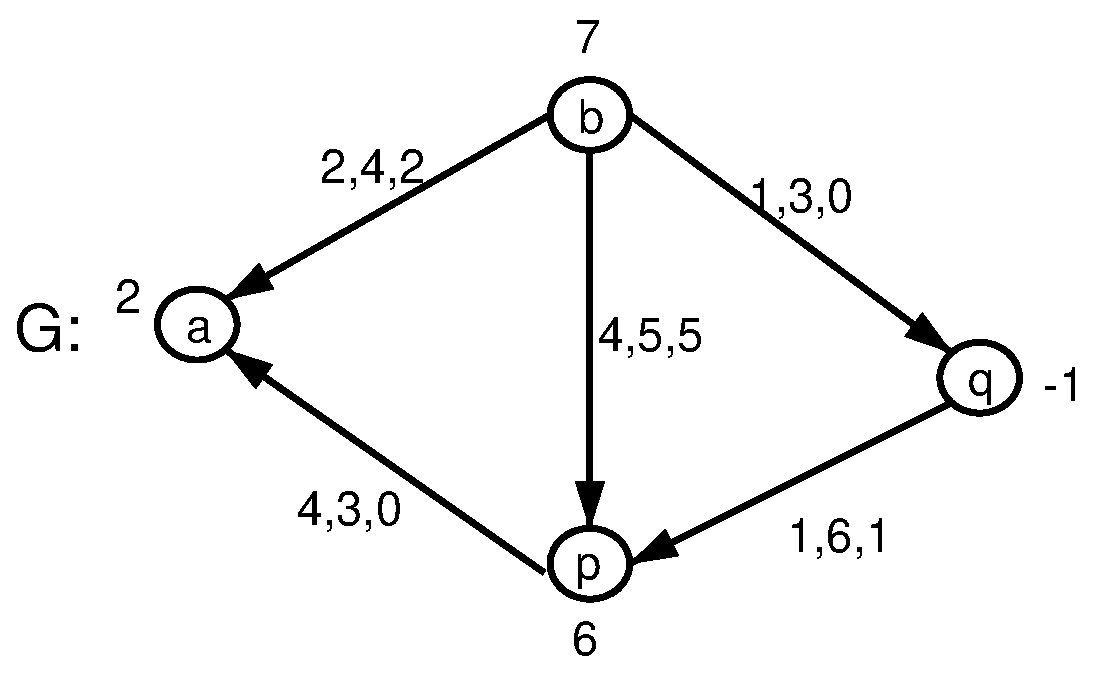
\includegraphics[width=6cm]{bilder/4-1Hilfsdigr1} \hspace{1cm} 
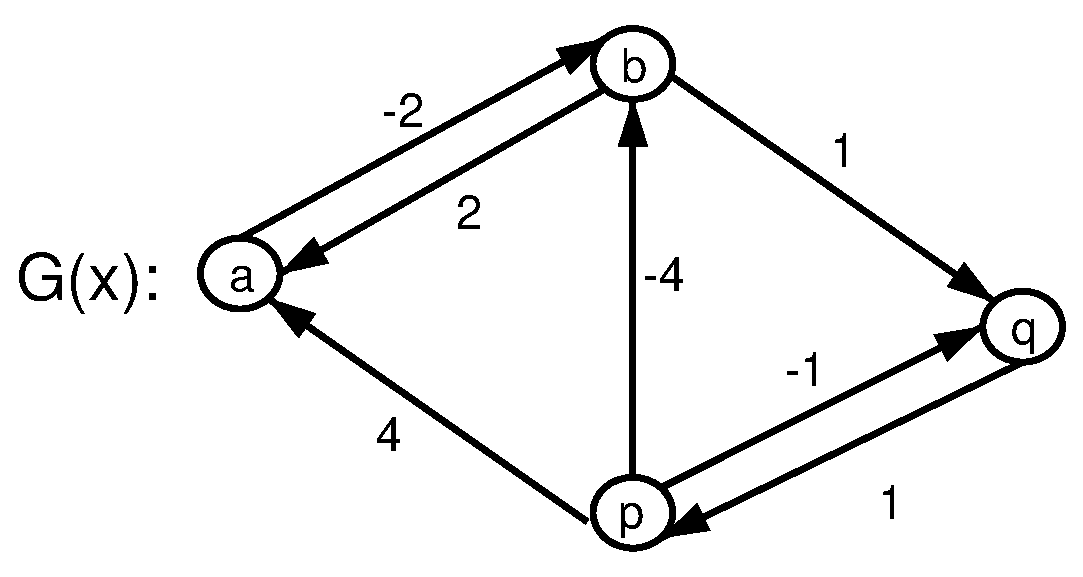
\includegraphics[width=6cm]{bilder/4-1Hilfsdigr2}

z.B. negativen Kreis $p b q$ um 3 erhöhen (Kostenminderung um 6):

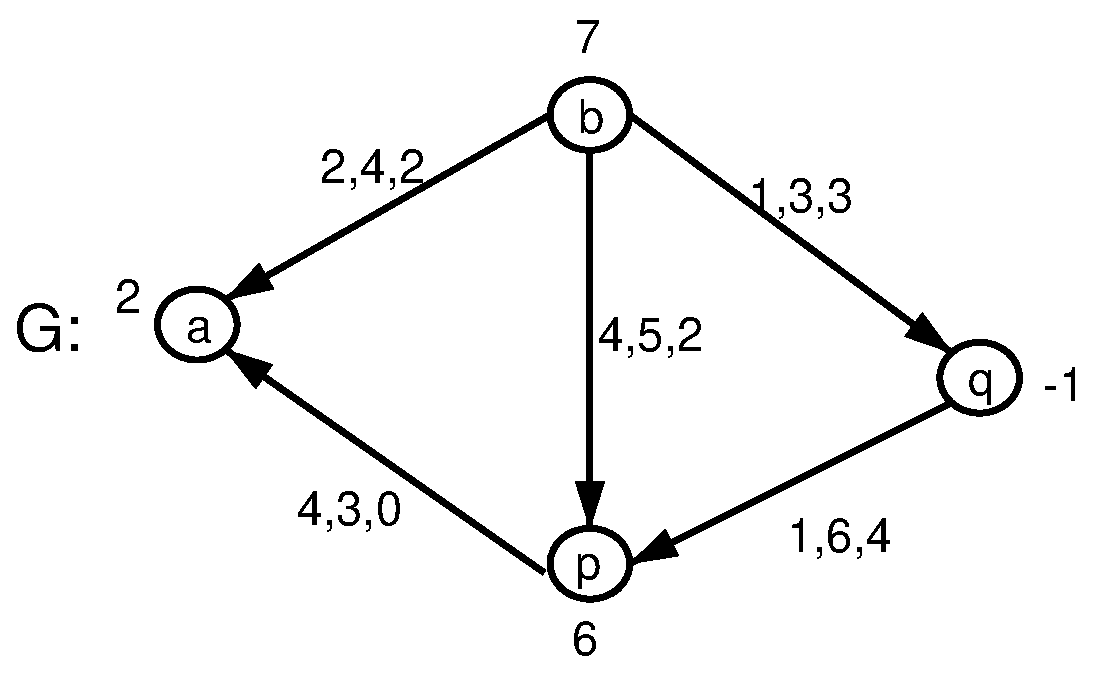
\includegraphics[width=6cm]{bilder/4-1Hilfsdigr3}

\begin{satz} \label{LösungLPMKFPopt}
Eine Zulässige Lösung $x$ von (LPMKFP) ist optimal g.d.w. kein
$x$-erhöhender Kreis mit neg. kosten existiert.
\end{satz}

Beweis:

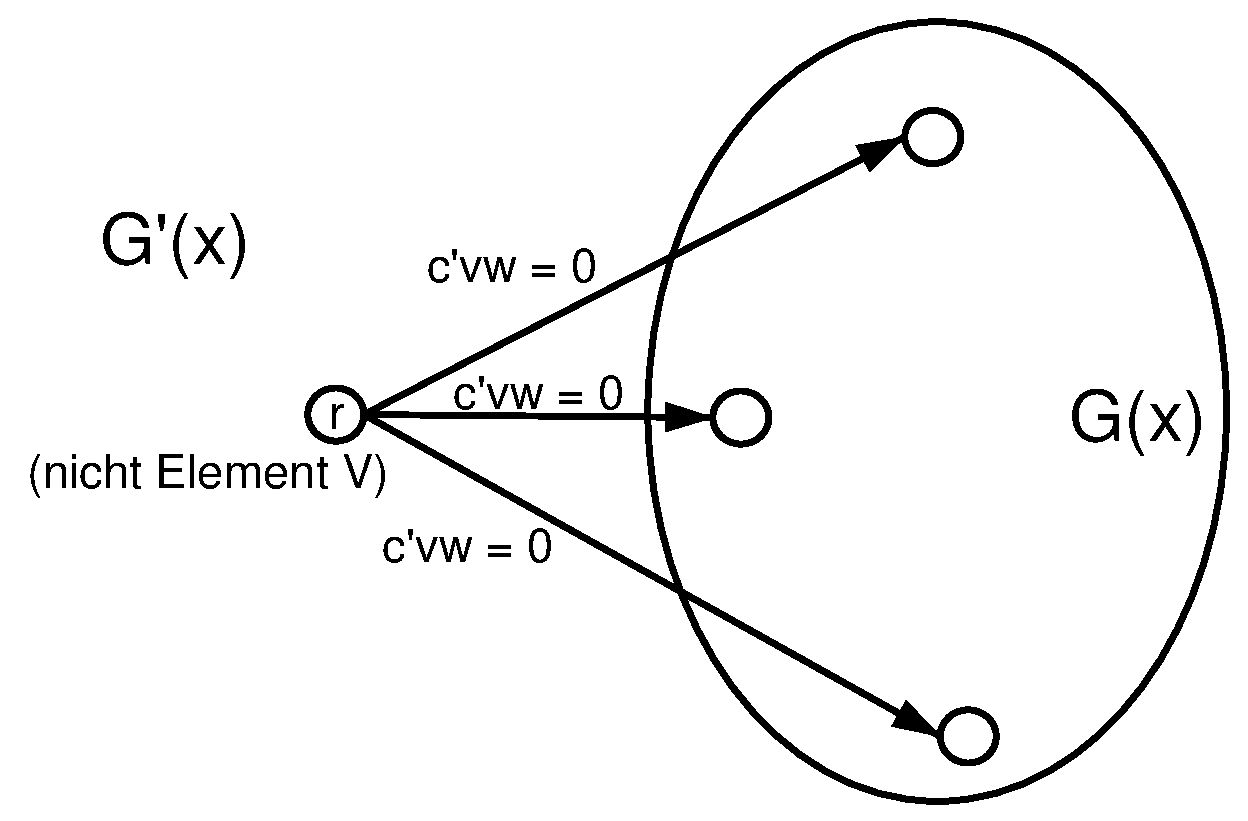
\includegraphics[width=7cm]{bilder/4-1BeweisSatz42}


Löse das kürzeste Wege Problem in $G'$.\\
Resultat: Entweder negativer Kreis oder zulässiges Potential:
\begin{enumerate}
\item Möglichkeit: Negativer Kreis: enthält $r$ nicht, liefert also
$x$-erhöhenden Kreis mit negativen Kosten.
\item Möglichkeit: zul. Potential:
\[\begin{array}{ll}
&y_{v} + c'_{v w} \geqq y_{w} \; \forall \; v w \in E(G(x))\\
\Leftrightarrow&\left\{\begin{array}{l}
y_{v} + c_{v w} \geqq y_{w} \mbox{ falls }x_{v w} < u_{v w}\\
y_{v} - c_{w v} \geqq y_{w} \mbox{ falls }x_{w v} > 0 \end{array} \right\}\\
\Leftrightarrow&\left\{\begin{array}{l}
x_{e} < u_{e} \Rightarrow \bar{c}_{e} \geqq 0\\
x_{e} > 0 \Rightarrow \bar{c}_{e} \leqq 0\end{array} \right\}
\mbox{\begin{tabular}{l}"`Konstruktion eines optimalen $y$\\ 
aus einem optimalen $x$"'\end{tabular}}\\
\Leftrightarrow & \left\{\begin{array}{l} \bar{c}_{e} < 0 \Rightarrow x_{e}
= u_{e}\\
\bar{c}_{e} > 0 \Rightarrow x_{e} = 0 \end{array} \right\} \hspace{2mm}
\mbox{Optimalitätsbed. aus Satz \ref{ZulLLPMKFP} q.e.d. }
\end{array}\]
\end{enumerate}

\begin{satz}
Hat (LPMKFP) eine Optimallösung und ist ganzzahlig, so kann $y$ in Satz
\ref{ZulLLPMKFP} ganzzahlig gewählt werden, d.h. (DLPMKFP) hat eine
ganzzahlige Optimallösung.
\end{satz}
Beweis:
Kantengewichte ganzzahlig $\Rightarrow$ Kürzeste Wege Kosten ganzzahlig
q.e.d.
\begin{satz} \label{LösungLPMKFPopt3}
hat (LPMKFP) eine zulässige Lösung so existiert eine Optimallösung genau
dann, wenn es keinen negativ gerichteten Kreis gibt, dessen Kapazitäten
alle unbeschränkt sind.
\end{satz}
Beweis:\\
"`$\Rightarrow$"' $\exists$ negativer Kreis$\ldots$ $\Rightarrow$ (LPMKFP)
unbeschränkt. trivial.\\
"`$\Leftarrow$'" $\nexists$ negativer gerichteter Kreis ...\\
Es reicht zu zeigen (DLPMKFP) hat zulässige Lösung $(y,z)$\\
Für $u_{e} \neq \infty$ wähle $z_{e} = \max\{0,-c_{e}\}$\\
Also brauchen wir $y$ mit $\bar{c}_{e} \geqq 0 \; \; \forall e$ mit $u_{e} =
\infty$

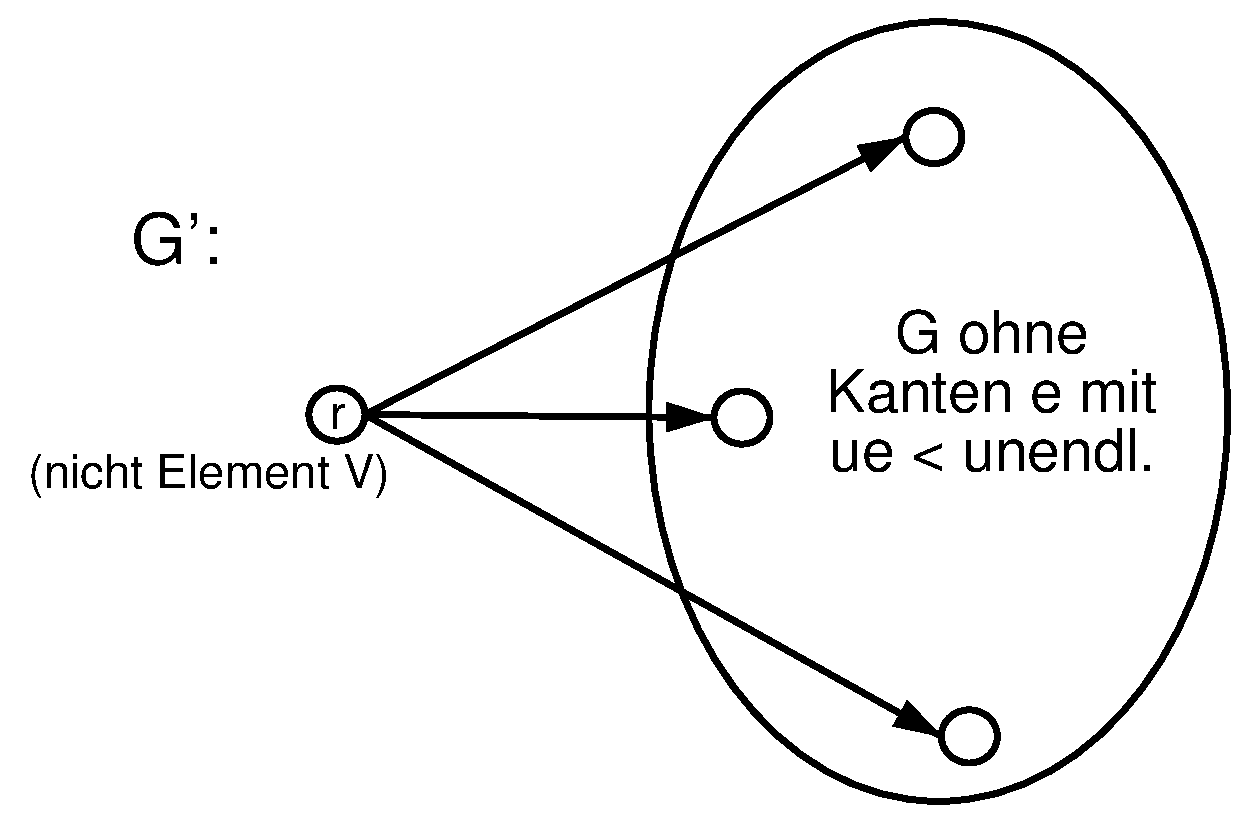
\includegraphics[width=8cm]{bilder/4-1BeweisSatz44}

wähle $y$ als zulässiges Potential in $G'$. q.e.d.

\paragraph{Konstruktion eines optimalen $x$ aus optimalem $y$} \mbox{}\\
Bedingungen für $x$:
\[(\ast)\left\{\begin{array}{l}
f_{x}(v) = b_{v} \; \; \forall \; v \in V\\
0 \leqq x \leqq u\\
\bar{c}_{e} > 0 \Rightarrow x_{e} = 0\\
\bar{c}_{e} < 0 \Rightarrow x_{e} = u_{e}
\end{array} \right.
\]
Definiere:
\[\begin{array}{rl}
u'_{e} = & \left\{ \begin{array}{l} 0 \mbox{ falls }\bar{c}_e > 0\\
u_{e} \mbox{ sonst}\end{array}\right.\\
l'_{e} = & \left\{ \begin{array}{l} u_{e} \mbox{ falls } \bar{c}_{e} < 0\\
0 \mbox{ sonst}\end{array}\right.\\
(\ast) \Leftrightarrow (\ast\ast)& \left\{ \begin{array}{l} f_{x}(v) =
b_{v}\\ l' \leqq x \leqq u'\end{array} \right.
\end{array}\]
Löse $(\ast\ast)$ mittels Maximum-Fluss-Algorithmus.

\begin{satz}
Sind $b$ und $u$ ganzzahlig und hat (LPMKFP) eine Optimallösung, so
existiert eine ganzzahlige Optimallösung. q.e.d.
\end{satz}

Reduktionen:
\begin{description}
\item[A] \[\begin{array}{rcll} \min c^{T}x\\
a_{v}\leqq f_{v}(x) &\leqq& b_{v} &\; \; \forall \; v \in V\\
l_{e} \leqq x_{e} &\leqq& u_{e} & \; \; \forall e \in E \end{array} \]
auf (MKFP)\\
Wir dürfen annehmen, dass
\item[A1] $(\forall \; v \in V) \; \; a_{v} = b_{v} $

\begin{tabular}{cc}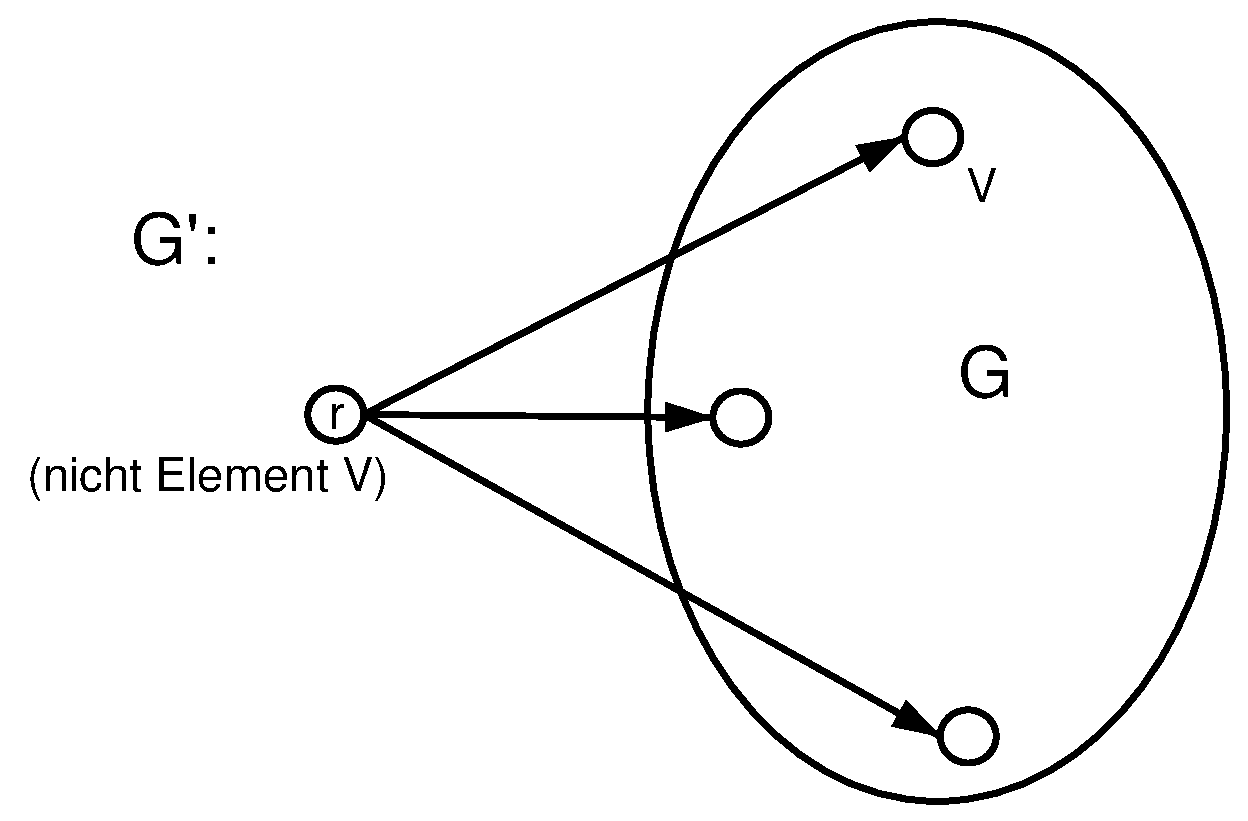
\includegraphics[width=8cm]{bilder/4-1Reduktion1}&
$\begin{array}[b]{lcl}
c_{r v} &=&0\\
l_{r v} &=& 0\\
u_{r v} &=& b_{v}- a_{v}\\
b_{r}&=& \displaystyle - \sum_{v \in V} b_{v}\\
\multicolumn{3}{l}{\mbox{Ersetze alle $a_{v}$ durch $b_{v}$}}
\end{array}$
\end{tabular}

im neuen Problem gilt:
\[\begin{array}{l}x_{r v} + f_{x}(v) = b_{r} \; \; \forall r \in V\\
\Rightarrow x_{r v} = b_{v} -f_{x}(v)\end{array}\]
D.h.:\\
\[\begin{array}{l}a_{v} \leqq f_{x}(v) \leqq b_{v} \Leftrightarrow 0 \leqq x_{r v} \leqq b_{v} -
a_{v}\\
\Leftrightarrow a_{v} \leqq b_{v} - \underbrace{x_{r v}}_{\geqq 0}
\underbrace{\leqq}_{\mbox{redundant}} l_{v}\\
\Leftrightarrow x_{r v} \leqq b_{v} - a_{v}
\end{array}\]
Zulässige Lösungen des neuen Problems eingeschränkt auf die alten Kanten
sind genau die zulässigen Lösungen des alten Problems:
\begin{itemize}
\item Gleicher ZF-Wert
\item $O(m)$ Kanten $O(n)$ Knoten, d.h. keinen Effizienzverlust
\end{itemize}
\item[A2] $(\forall \; e \in E) \; l_{e} \neq -\infty$ oder $u_{e} \neq
\infty$\\ Dies wird eine Übungsaufgabe sein!
\item[A3] $(\forall \; e \in E)\;  l_{e} \neq \infty$\\
Nach A2 gilt: $l_{e} = -\infty \Rightarrow u_{e} \neq \infty$\\
Ersetze $v\stackrel{e}{\rightarrow}w$ durch $v\stackrel{e'}{\leftarrow}w$
\[\begin{array}{lcl}
c_{e'}&=& -c_{e}\\
l_{e'} &=& -u_{e}\\
u_{e'} &=& \infty
\end{array}\]
\item[A4] $(\forall \; e \in E)\; l_{e} = 0$\\
$u_{e} := u_{e} - l_{e}$\\
$\begin{array}{rcl}(e=vw) \; b_{v} &:=& b_{v} + l_{e}\\
b_{w} &=& b_{w} - l_{e} \end{array}$\\
$l_{e} := 0$

\begin{tabular}{llc}
vorher:&$\overbrace{v}^{b_{v}}\stackrel{l_{e}\leqq x_{e} \leqq
u_{e}}{\longrightarrow}\overbrace{b_{w}}^{b_{w}}$& Fluss mit Kosten $k$\\
nachher:&$\overbrace{v}^{b_{v}+l_{e}}{v}\stackrel{0\leqq x_{e} - l_{e} \leqq
u_{e} - l_{e}}{\longrightarrow}\overbrace{w}^{b_{w}-l_{e}}$& Fluss mit Kosten
$k - c_{e} l_{e}$\end{tabular}
\item[B] (MKFP) auf das Transshipment\\
$v\stackrel{c_{e}, \; u_{e} \neq \infty}{\longrightarrow} w \; \; \;
\rightarrow \;\; \; v
\stackrel{c_{e},\, \infty}{\longrightarrow}p\stackrel{0,\;
\infty}{\longleftarrow}q\stackrel{0,\, \infty}{\longrightarrow}w$ mit
$b_{p} = u_{e}$ und $b_{q} = -u_{e}$ \\
Vor der Umwandlung $O(m+n)$ Knoten und $O(m)$ Kanten. Nach der Umwandlung
$O(n+2m)$ Knoten und $O(3m)$ Kanten. Das ist in der Praxis ineffizient,
aber genug um zu zeigen, dass gewisse Algorithmen polynomiell sind.
\end{description}

\section{Primale Minimum Kosten Fluss Algorithmen}
\subsection{Basis-Algorithmus}
Dieser Algorithmus stammt von Kanorovich [1942]. Er läuft so:\\
\begin{algorithmic}
\STATE Finde eine zulässige Lösung $x$;
\WHILE{($\exists$ $x$-erhöhender Kreis mit negativen Kosten)}
\STATE Finde einen $x$-erhöhenden Kreis $C$ mit negativen Kosten;
\IF{($C$ hat keine Rückwärtskanten und keine Vorwärtskanten mit endl.
Kapazität)}
\STATE STOP "`unbeschränkt"';
\ENDIF
\STATE Augmentiere $x$ auf $C$;
\ENDWHILE
\end{algorithmic} 

Dabei stellt sich die Frage, wie viele Flusserhöhungen durchgeführt
werden.\\
Max-Fluss-Problem als spezielles MKFP

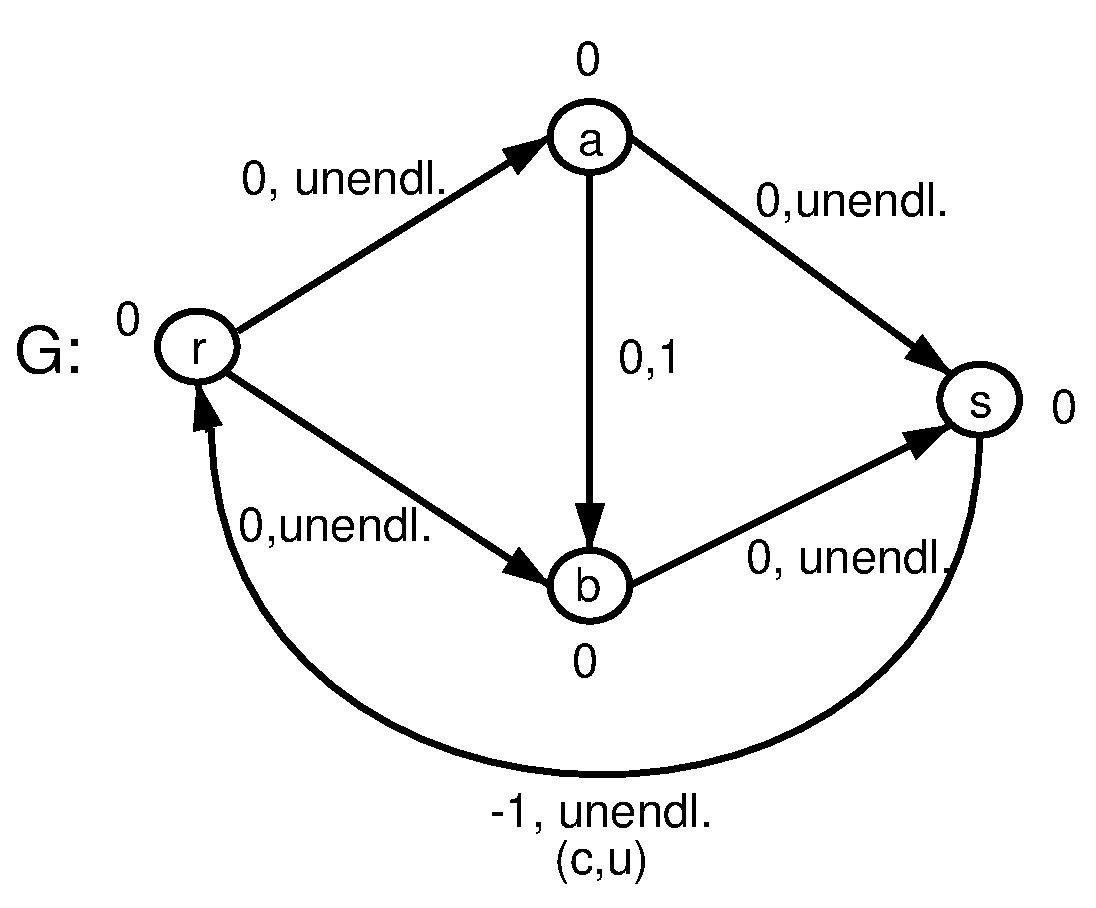
\includegraphics[height=4cm]{bilder/4-2MaxFlussalsMKFP}

$x$-erhöhende Wege $\entspricht$ negative Kreise.\\
$\Rightarrow$ evtl. keine Terminierung.

\paragraph{Abhilfe} Max-Fluss: Kürzeste augmentierende Wege\\
hier: "`negativste"' Kreise?\\
nein: die Kreise im Beispiel sind "`negativst"', stattdessen:\\
minimale Durchschnittskosten für Kreis $C$
\[ := \frac{\mbox{Kosten }C}{\mbox{Länge }C}\]
$\entspricht$ kürzeste Wege im Max-Fluss.\\
Zeit pro Iteration $O(m n)$ mit Bellmann Ford $\leftarrow$ zu teuer\\
aber: ergibt polynomiellen Algorithmus (nach Goldberg u. Tarjan [1989])

\subsection{Die Netzwerk-Simplex Methode}

Erinnerung: Satz \ref{Spaltenb-Baum}: Spaltenbasen entsprechen eins zu eins
den aufspannenden Bäumen.

Hier anderer Zugang: Spezialisierung des Basis-Algorithmus.
Annahme: $G$ ist zusammenhängend (OBdA: sonst Zusammenhangs-Komponenten 
getrennt behandeln)

$\rightarrow G$ hat aufspannenden Baum (ab jetzt genannt Baum)\\
Zunächst Spezialisierung auf das Transshipment-Problem. ($u_{e} = \infty \;
\forall \; e \in E)$

Baum-Lösung $x \in \RR^{E}$ mit:
\[\begin{array}{rcll} f_{x}(v) &= &b_{v} &\; \; \forall v \in V\\
x_{e}&=&0 &\; \; \forall \; e \not\in T \end{array}\]
für einen Baum $T$

\begin{lemma}
Zu je zwei Knoten $u$ und $v$ eines Baumes $T$ existiert ein eineindeutiger
$(u,v)$-Weg in $T$. Beweis klar. q.e.d
\end{lemma}

\begin{lemma}
Ein Baum $T$ bestimmt eindeutig seine Baumlösung.
\end{lemma}

Beweis:\\
$r \in V(T)$ beliebig fest "`Wurzel"'\\
$h=p q \in E(T)$\\
$R(T,h) = \{v \in V(T) | \mbox{eindeutiger $(r,v)$-Weg in T benutzt $h$
nicht}\}$

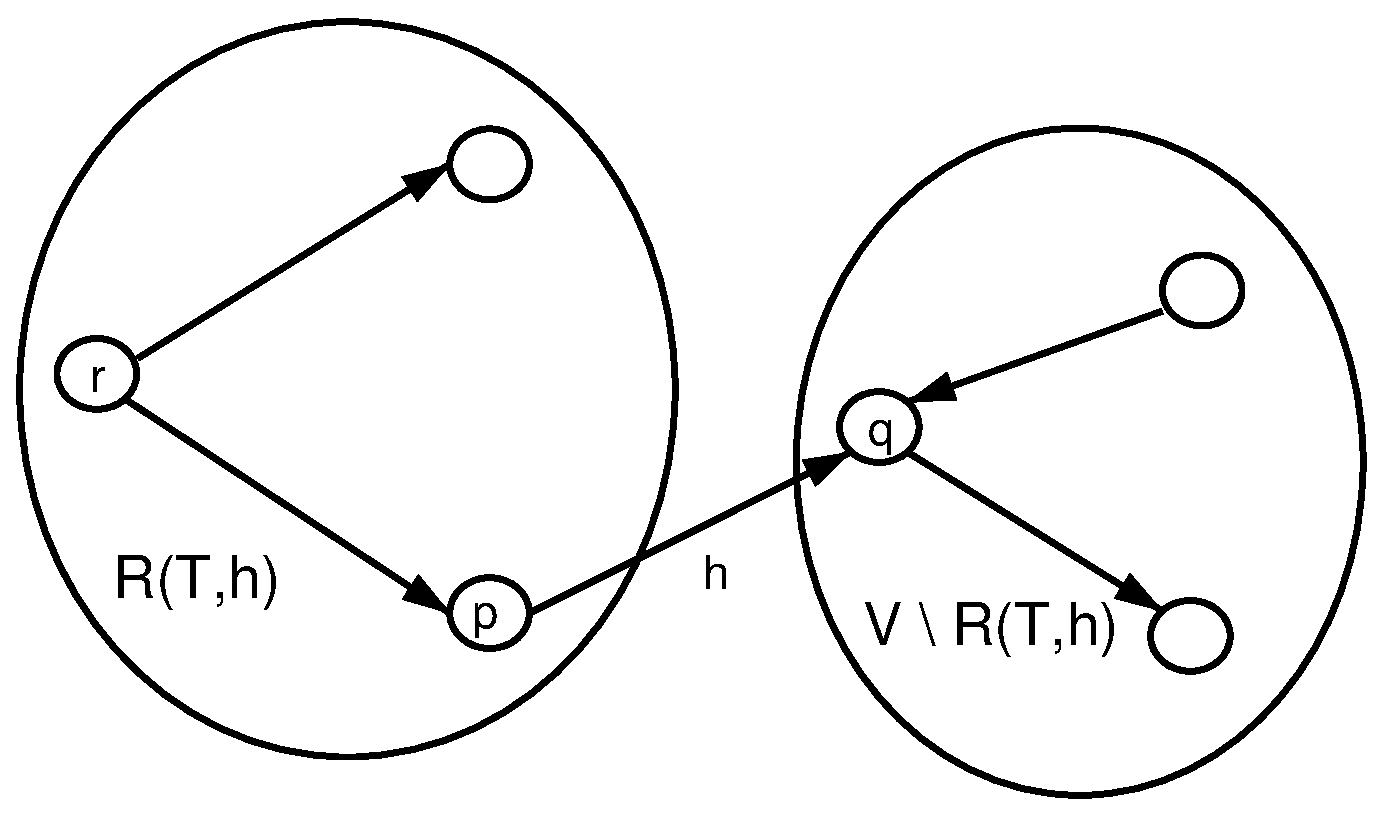
\includegraphics[height=4cm]{bilder/4-2BeweisL47}

$\Rightarrow x_{h} = \left\{\begin{array}{ll}-b(R(T,h)) \mbox{ falls } p
\in R(T,h)\\ b(R(T,h)) \mbox{ falls } q \in R(T,h)\end{array}\right.
\mbox{q.e.d.}$\\
Die Umkehrung gilt nicht, z.B. alle $b_{v} = 0 \Rightarrow$ alle
Baumlösungen $\entspricht x=0$

\begin{satz}
Hat $(G,b)$ eine zulässige Lösung, so auch eine zulässige Baumlösung, hat
$(G,b)$ eine optimale Lösung, so auch eine optimale Baumlösung.
\end{satz}
Beweis: Sei $x$ eine zulässige Lösung, aber keine Baumlösung\\
$\Rightarrow \exists$ Kreis $C$ mit positivem Fluss auf jeder Kante (OBdA
habe $C$ eine Rückwärtskante, sonst wähle $C$ anders herum).

$\epsilon := \min \{x_{e} | e \mbox{ ist Rückwärtskante} \}$
$x_{e} \rightarrow \left\{ \begin{array}{ll} x_{e} + \epsilon \mbox{ falls $e$
Vorwärtskante in $C$}\\
x_{e}-\epsilon  \mbox{ falls $e$ Rückwärtskante in $C$} \end{array}
\right.$

Resultat: Ein neues zulässiges $x$ mit weniger Kanten mit positivem Fluss\\
Schließlich: Baumlösung

Jetzt $x$ optimale Lösung, Kreis $C$ mit positivem Fluss.\\
Aus Satz \ref{LösungLPMKFPopt}: (zulässiges $x$ ist optimal g.d.w. kein
neg. Kreis)
$\Rightarrow C$ hat Kosten 0\\
Weiter wie oben 

\subsubsection{Grundidee der Netzwerk-Simplex-Methode}
\begin{itemize}
\item Erzeuge Eine Folge von Baumlösungen
\item Suche nach speziellen negativen Kreisen zu jeder Kante $e=v w \not\in
T$ existiert ein eindeutiger Kreis C(T,e) mit:
\begin{itemize}
\item $f \in C(T,e) \rightarrow f \in T \cup \{e\}$
\item $e$ ist Vorwärtskante in $C(T,e)$
\item Der "`Anfangsknoten"' $s$ von $C(T,e)$ ist der erste gemeinsame
Knoten der einfachen $(v,r)$- und $(w,r)$-Wege in $T$
\end{itemize}
\end{itemize}

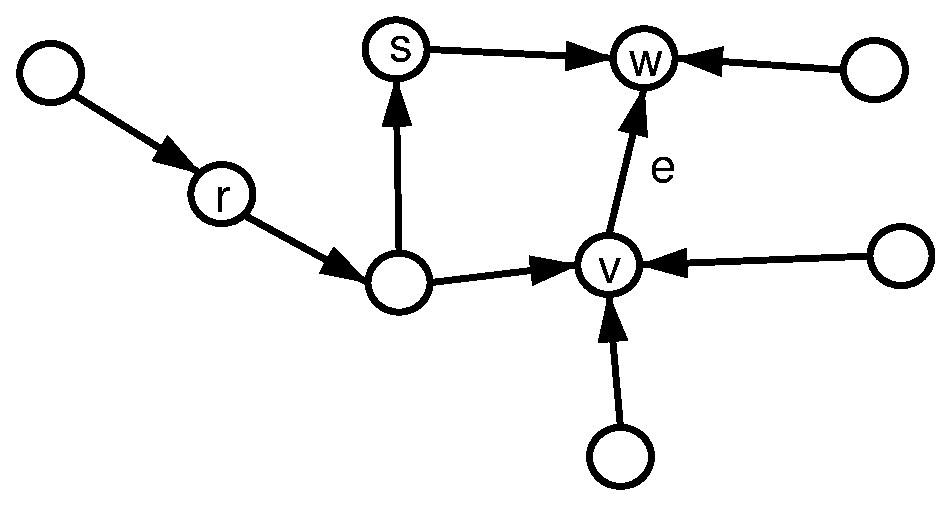
\includegraphics[height=3cm]{bilder/4-2NetzSimpl1}

\begin{satz}\label{NSBaumopt}
Definiert der Baum $T$ die zulässige Baumlösung und hat $C(T,e)$
nicht-negative Kosten für alle $e \not \in T$, so ist $x$ optimal.
\end{satz}
Beweis: Sei $y\in \RR^{V}$ mit $y_{v} =$ Kosten des einfachen $(r,v)$-Wege
in $T$. Für alle $v,w \in V$ gilt: Kosten des einfachen $(v,w)$-Wege
$=y_{w} - y_{v}$.

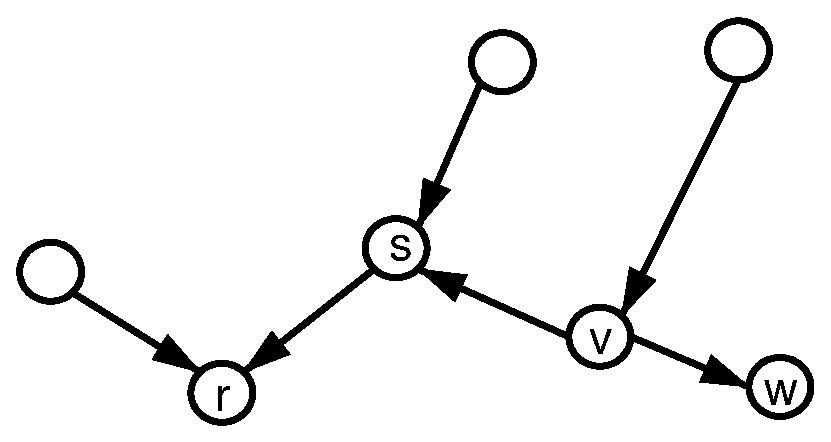
\includegraphics[height=3cm]{bilder/4-2NetzSimpl2}

Also gilt für die reduzierten Kosten: $\bar{c}_{v w} = c_{v w } + y_{v} -
y_{w}$\\
falls $v w \in T$: $\bar{c}_{v w} = c_{v w} + y_{v} - y_{w} = y_{w} - y_{v}
+ y_{v}-y_{w} = 0$\\
$\mbox{falls }v w \in E \wout T: \; \bar{c}_{v w} \begin{array}[t]{l}= \underbrace{c_{v
w}}_{\mbox{\small Kosten $v w$}} + \underbrace{y_{v} -y_{w}}_{\mbox{\small Kosten im Baum
von $w$ nach $v$}}\\ =$ Kosten von $C(T, v w) \geqq 0\end{array}$
 
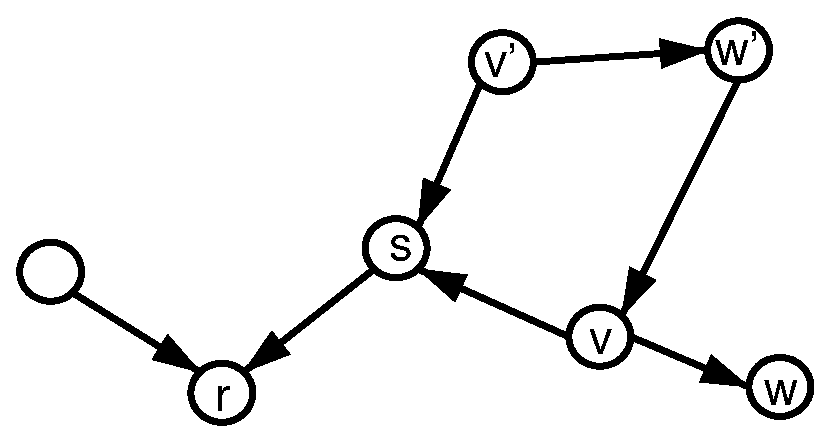
\includegraphics[height=3cm]{bilder/4-2NetzSimpl3}

D.h. die Bedingung von Satz \ref{ZulLLPMKFP} (Komplementärer Schlupf
$\bar{c}_{e} > 0 \Rightarrow x_{e} = 0$) sind erfüllt.
$\stackrel{\mbox{\footnotesize Satz \ref{ZulLLPMKFP}}}{\Rightarrow}$ Optimalität.

Test ob $T$ diese Optimalitätsbedingungen erfüllt:\\
$\left.\begin{array}{l}
\mbox{- Berechne $y$: Zeit $O(n)$}\\
\mbox{- Berechne $\bar{c}$: Zeit $O(m)$}\end{array} \right\}
\mbox{Besser als $O(m n)$ für Bellmann-Ford aber:}$\\
Problem: Verbessert $C(T,e)$ die Lösung?\\
$C(T,e)$ kann eine Rückwärtskante mit 0-Fluss haben.

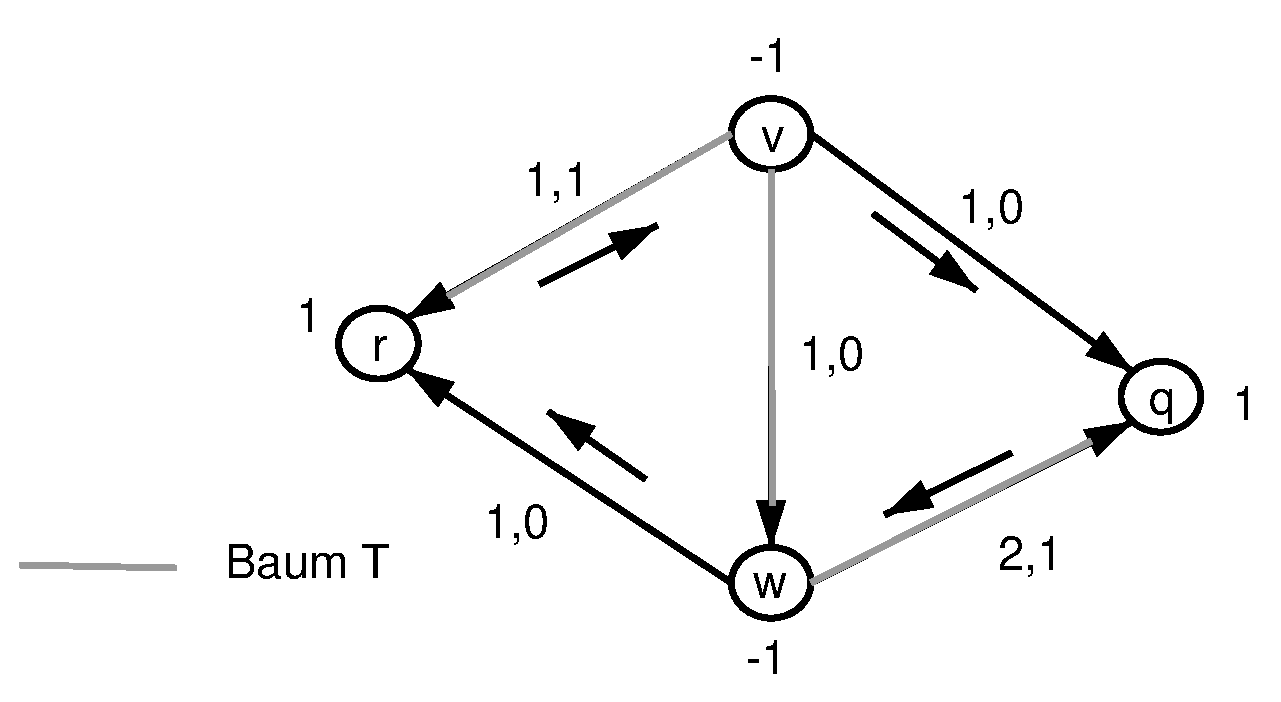
\includegraphics[height=3cm]{bilder/4-2NetzSimpl4}

$C(T,w r)$ hat positive Kosten 1.\\
$C(T, v q)$ hat negative Kosten -2, aber Rückwärtskante $v w $ mit
0-Fluss.\\ Aber $x$ ist nicht optimal.\\
Eine Einheit Fluss auf dem durch die kurzen Pfeile markierten Kreis liefert
eine bessere Lösung (um -1).

Trotzdem:

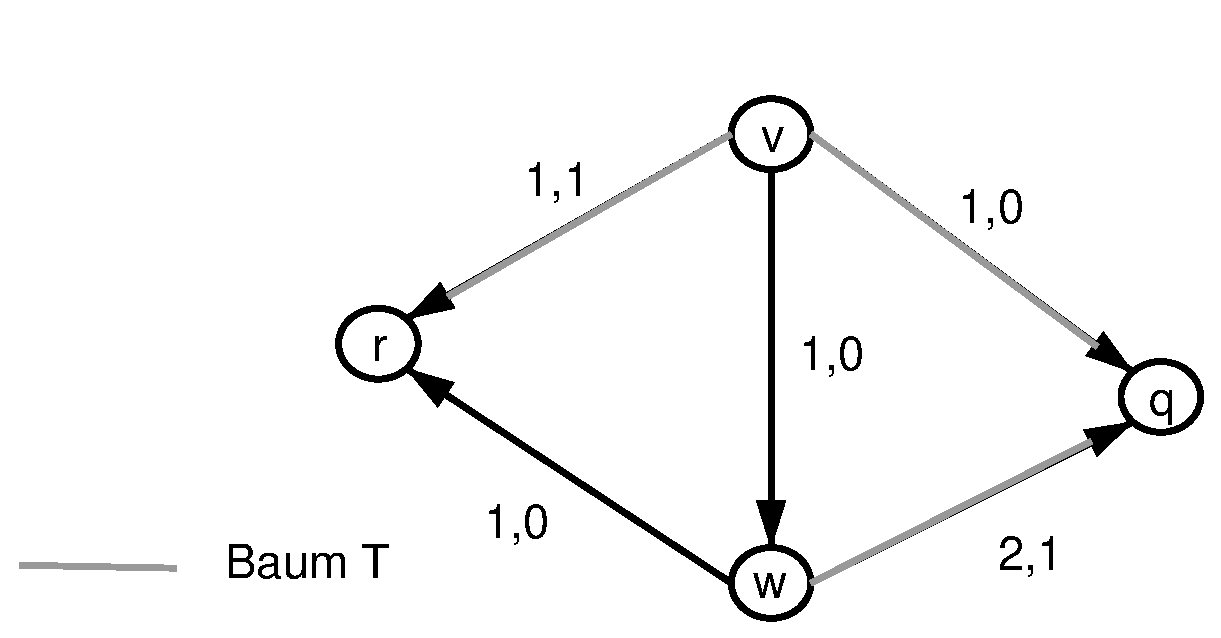
\includegraphics[height=3cm]{bilder/4-2NetzSimpl5}


\subsubsection{Netzwerk-Simplex-Algorithmus für das 
Transshipment-Problem}

\begin{algorithmic}
\STATE Finde Baum $T$ mit zulässiger Baumlösung $x$;
\STATE Berechne für alle $v\in V$ $y_{v} =$ Kosten des $(r,v)$-Weges in
$T$;
\WHILE{($\exists e = v w$ $(e\not\in T)$ mit $\bar{c}_{e} = c_e+ y_{v} - y_{w} < 0$)}
\STATE Finde solches $e$;
\IF{($C(T,e)$ hat keine Rückwärtskante)}
\STATE STOP unbeschränkt;
\ENDIF
\STATE Berechne $\Theta = \min\{x_{j} | j \mbox{ rückwärts in } C(T,e)\}$
\STATE Bestimme Rückwärtskante $h$ von $C(T,e)$ mit $x_{h} = \Theta$;
\STATE Augmentiere $x$ um $\Theta$ auf $C(T,e)$;
\STATE Setze $T := (T \cup \{e\}) \wout \{h\}$;
\STATE Berechne neue $y$;
\ENDWHILE
\end{algorithmic}

Erzeugung eines ersten Baumes (Initialisierung):

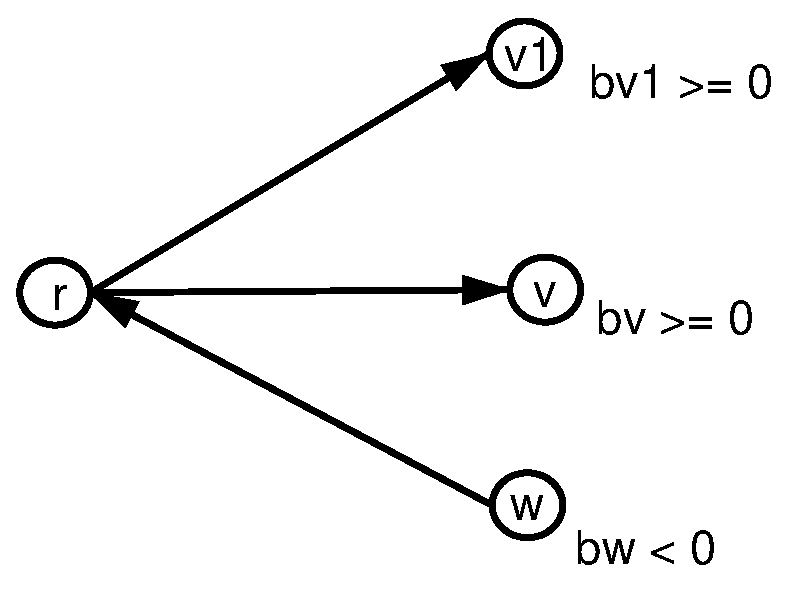
\includegraphics[height=3.5cm]{bilder/4-2NetzSTrans}

Künstliche Kanten, Hohe kosten $M$ falls $\not\in G$\\
$M := n\cdot \max\{|c_{e}|:\;  e \in E\} + 1$

\begin{lemma}\label{EntfNetzS}
Sei $T$ der alte $\hat{T}$ der neue Baum, so gilt für $e=v w$:
\[\hat{y}_{q} = \left\{ \begin{array}{ll}
y_{q} & \forall \; q \in R(T,h)\\
y_{q} + \bc_{e} & \forall \; q \not\in R(T,h) \mbox{, falls } v \in
R(T,h)\\
y_{q} - \bc_{e} & \forall q \not\in R(T,h)  \mbox{, falls } w \in R(T,h) 
\end{array}\right.\]
\end{lemma}
Beweis:

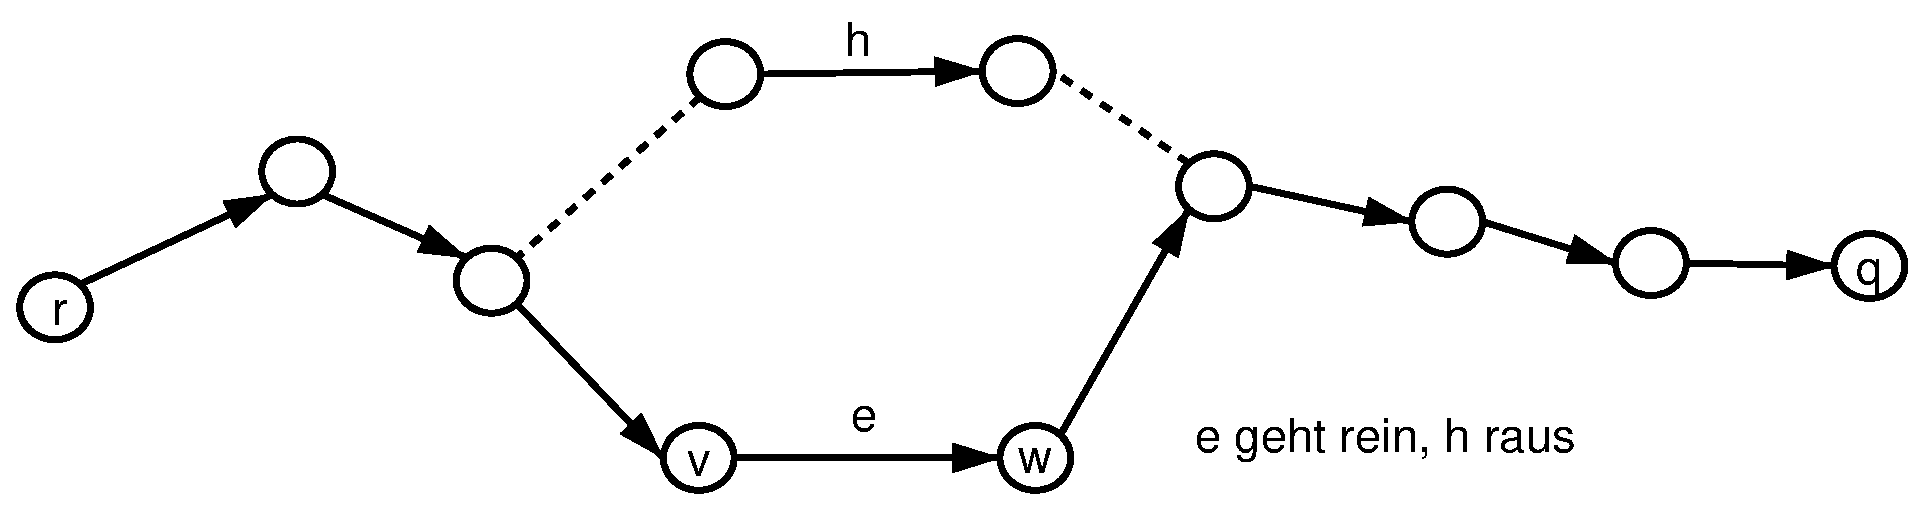
\includegraphics[height=3cm]{bilder/4-2NetzSTransB}

für $q \in R(T,h)$: gleicher Weg $\rightarrow$ gleiche Kosten\\
für $q \not\in R(T,h)$ und $v \in R(T,h)$\\
\[\begin{array}{rcl}
\hat{y}_{q} &= &y_{v} + c_{e} + (y_{q}-y_{w})\\
&=& y_{q} + \bar{c}_{e}\end{array}
\]
für $q \not\in R(T,h)$, $w\in R(T,h)$ analog. q.e.d.

\subsubsection{Endlichkeit des Netzwerk Simplex-Algorithmus}

Sei $T$ Baum mit 0-Flusskante ist {\em degeneriert} (hat 0-Kante), dann ist
Zykeln möglich (Übungsaufgabe), aber vermeidbar. Dafür zunächst eine
Definition:\\
$h=p q \in T$ ist {\em von} $r$ gerichtet, falls $p \in R(T,h)$\\
$h=p q \in T$ ist {\em auf} $r$ gerichtet, falls $q \in R(T,h)$

$T$ ist {\em stark zulässig} falls für den zugehörigen Fluss gilt:\\
$\forall \; h \in T$ mit $x_{h} =0$ ist $h$ von $r$ gerichtet.\\ 

Jeder nicht degenerierte Baum und der Anfangsbaum sind stark zulässig.

C-Regel: Wähle $h$ als {\em erste} Rückwärtskante von $C(T,e)$ mit $x_{h} =
\Theta$. Diese Regel wurde 1976 von Cunningham aufgestellt.

\begin{lemma}
Ist $T$ stark zulässig und entsteht $\hat{T}$ aus $T$ mit der C-Regel, so
ist auch $\hat{T}$ stark zulässig.
\end{lemma}
Beweis: Situation $Ee$ rein, $h$ raus, $x$ alter, $\hat{x}$ neuer Fluss.
\begin{enumerate}
\item $g\not \in C(T,e)$\\
$g$ von $r$ in $\hat{T} \Leftrightarrow g$ ist von $r$ in T:\\
$\hat{x}_{g} = x_{g}$
\item $g \in C(T,e)$
\begin{enumerate}
\item $\Theta > 0$:\\
$\hat{x}_{g} = 0 \Leftrightarrow$ rückwärts in $C(T,e)$ und $x_{q} =
\Theta$\\
$h$ ist erste von diesen

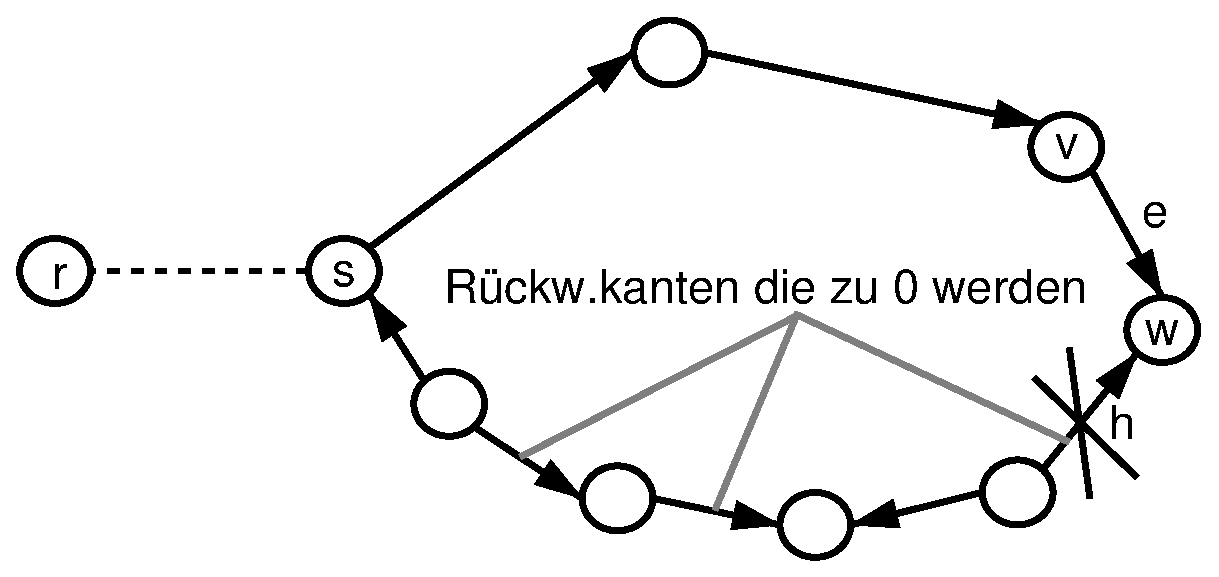
\includegraphics[height=3cm]{bilder/4-2NetzSTransB2}

Es wird $h$ genommen $\Rightarrow$ alle anderen sind von $r$.
\item $\Theta = 0$\\
$\hat{x}_{g}=0$ g.d.w. $x_{g} = 0 $ (incl. $\hat{x}_{e} = 0$)\\
$T$ stark zulässig $\Rightarrow$ alle diese außer $e$ vorwärts in $(s,v)$
und $(s,w)$-Wegen in $T$. Letzter von diesen wird gewählt.\\
$ \Rightarrow$ alle anderen sind von $r$ in $\hat{T}$\\
$e$ ist vorwärts in $C(T,e) \Rightarrow e$ von $r$ in $\hat{T}$\\
$\Rightarrow \hat{T}$ ist stark zulässig q.e.d.\\
\end{enumerate}
\end{enumerate}
\begin{satz}
Startet der Netzwerk-Simplex-Algorithmus mit einem stark zulässigen Baum
und benutzt er die C-Regel, so terminiert er.
\end{satz}
Beweis: Wir zeigen: Zykeln unmöglich.

Sei $\begin{array}{c}T\\(y)\end{array} \stackrel{h\mbox{ raus, } e 
\mbox{ rein}}{\Longrightarrow} \begin{array}{c}\hat{T}\\(\hat{y})\end{array}$
degenerierte Iteration.

$h$ sei Vorwärtskante auf $(s,w)$-Weg.
\[R(T,h)\stackrel{h}{\rightarrow}\ldots\rightarrow w\]
$\Rightarrow w \not\in R(T,h) \Rightarrow v \in R(T,e)$\\
$\stackrel{\ref{EntfNetzS}}{\Rightarrow} \hat{y}_{w} = y_{w}+
\underbrace{\bc_{e}}_{< 0} < y_{w}$\\
$\Rightarrow \hat{y}_{a} \leqq y_{a} \; \; \forall\; a \in V$ und
$\hat{y}_{w} < y_{w}$\\
$\Rightarrow \displaystyle \sum_{a\in V} \hat{y}_{a} < \sum_{a \in V}
y_{a}$\\
$\Rightarrow$ keine Wiederholung derselben Situation. q.e.d.

\subsubsection{Generalisierung von Transshipment auf Minimum Fluss}
(Skizze) analog Simplex-Algorithmus mit unteren und oberen Schranken.\\
Baum-Lösung: $x\in \RR^{E} \; \; \exists$ Baum $T$ und eine Partition (L,U)
von $E \wout T$ mit:
\[\begin{array}{lcl}
f_{x}(v)&=& b_{v}\\
x_{e}&=&0 \; \; \forall \; e \in L\\
x_{e} &=& u_{e} \forall \; e \in U;  
\end{array}\]
\begin{satz}
Hat $(G,b,u)$ eine zulässige (b.z.w optimale) Lösung so auch eine zul.
(b.z.w. optimale) Baumlösung
\end{satz}

Beweis analog. q.e.d.

Iteration wie vorhin, aber wenn $x_{e} = u_{e}$ dann Kreis andersherum ($e$
rückwärts).

Gegeben: $(T,L,U)$, $e \in L \cup U$\\
Kreis $C(T,L,U,e)$:\\
\begin{itemize}
\item Kanten alle aus $T\cup\{e\}$
\item $e$ vorwärts, falls $e \in L$, sonst rückwärts
\item Anfangsknoten $s$ wie gehabt.
\end{itemize} 
$y_{v}$ $(v\in V)$ wie gehabt, Kosten von $C(T,L,U,e) = \left\{\begin{array}{rl}
\bc_{e}&\mbox{falls }e \in L\\-\bc_{e}&\mbox{falls }e \in U \end{array}\right. $

Analogon zu Satz \ref{NSBaumopt}:
\begin{satz}
Definiert der Baum $(T,L,U)$ die zul. Baumlösung $x$ und hat $C(T,L,U,e)$
nicht-negative Kosten für alle $e\not\in T$, so ist $x$ optimal.
\end{satz}

\subsubsection{Netzwerk-Simplex-Methode für Minimum-Kosten-Flussprobleme}

\begin{algorithmic}
\STATE Finde Baum $(T,L,U)$ mit zul. Baumlösung;
\STATE Berechne für alle $v \in V \; \; y_{v} =$ Kosten eines $(r,v)$-Weges
in $T$;
\WHILE{($\exists e = v w \in L$ mit $\bc_{e} < 0$ oder $\exists e \in U$ mit
$\bc_{e} > 0$)}
\STATE Finde ein solches $e$;
\IF{($C(T,L,U,e)$ hat keine Rückwärtskante und keine Vorwärtskante endl.
Kapazität)} 
\STATE STOP "`unbeschränkt"';
\ENDIF
\STATE Berechne $\begin{array}[t]{l}\Theta_{1} := \min\{x_{j}|j \mbox{
rückwärts in }C(T,L,U,e)\}\\
\Theta_{2} := \min\{u_{j} -x_{j}|j \mbox{ vorwärts in }C(T,L,U,e)\}\\
\Theta := \min\{\Theta_{1}, \, \Theta_{2}\};\\
\end{array}$
\STATE Finde $h \in C(T,L,U,e)$ mit $h$ rückwärts und $x_{h} = \Theta$ oder
$h$ vorwärts und $u_{e} - x_{h} = \Theta$;
\STATE Augmentiere $x$ um $\Theta$ auf $C(T,L,U,e)$;
\STATE $T := (T \cup \{e\}) \wout \{h\}$;
\STATE Berechne neues $L$ und neues $U$;
\STATE Berechne neues $y$;
\ENDWHILE
\end{algorithmic}

Stark zulässige Baumlösung $T,x$:\\
$\forall \; e \in T$ mit $x_{e} =0$ ist $e$ von $r$ gerichtet\\
$\forall \; e \in T$ mit $x_{e} =u_{e}$ ist $e$ auf $r$ gerichtet

C-Regel: Wähle erste mögliche Kante

\section{Primal-Duale min Kosten Flussalgorithmen}

Idee: In jeder Iteration haben wir ein Paar $(x,y)$ mit $0 \leqq x \leqq u$
und Optimalitätsbedingungen aus Satz \ref{ZulLLPMKFP}:
\[
\begin{array}{l}
x_{e}=u_{e} \; \; \forall \; e \in E \mbox{ mit } \bc_{e} < 0\\
x_{e}=0 \; \; \forall \; e \in E \mbox{ mit }\bc_{e} > 0
\end{array}
\]
Zusammen mit $0 \leqq x \leqq u$ sind dies die Primal-Dual-Bedingungen.

Ziel: Erfüllung der Flussbedingungen:
\[f_{x}(v)=b_{v} \; \; \forall \; v \in V\]

Erste Lösung:\\
$c \geqq 0: \; x=0, \; y = 0$\\
sonst Lösen des kürzesten Wege-Problems wie in Satz
\ref{LösungLPMKFPopt3}.\\
Resultat: Entweder $\nexists$ Optimallösung oder $y$ mit $\bc_{e} \geqq 0$
wenn $u_{e} = \infty$

Wähle $\begin{array}[t]{ll}x_{e} = u_{e} & \mbox{falls } \bc_{e} < 0\\
x_{e} = 0& \mbox{sonst}\end{array}$ 

Also: Anfangslösung kann durch höchstens eine kürzeste Wege-Berechnung
ermittelt werden.\\
Und Existenz einer Lösung: Max-Fluss-Problem\\
Ab jetzt (OBdA): Existenz einer Optimallösung gesichert.

$v \in V$ heißt \begin{tabular}[t]{lll}$x$-Quelle,&falls $b_{v} <f_{x}(v)$& 
"`zu viel Fluss"'\\
$x$-Senke,&falls $b_{v} > f_{x}(v)$&"`zu wenig Fluss"'\end{tabular} 


Beispiel:

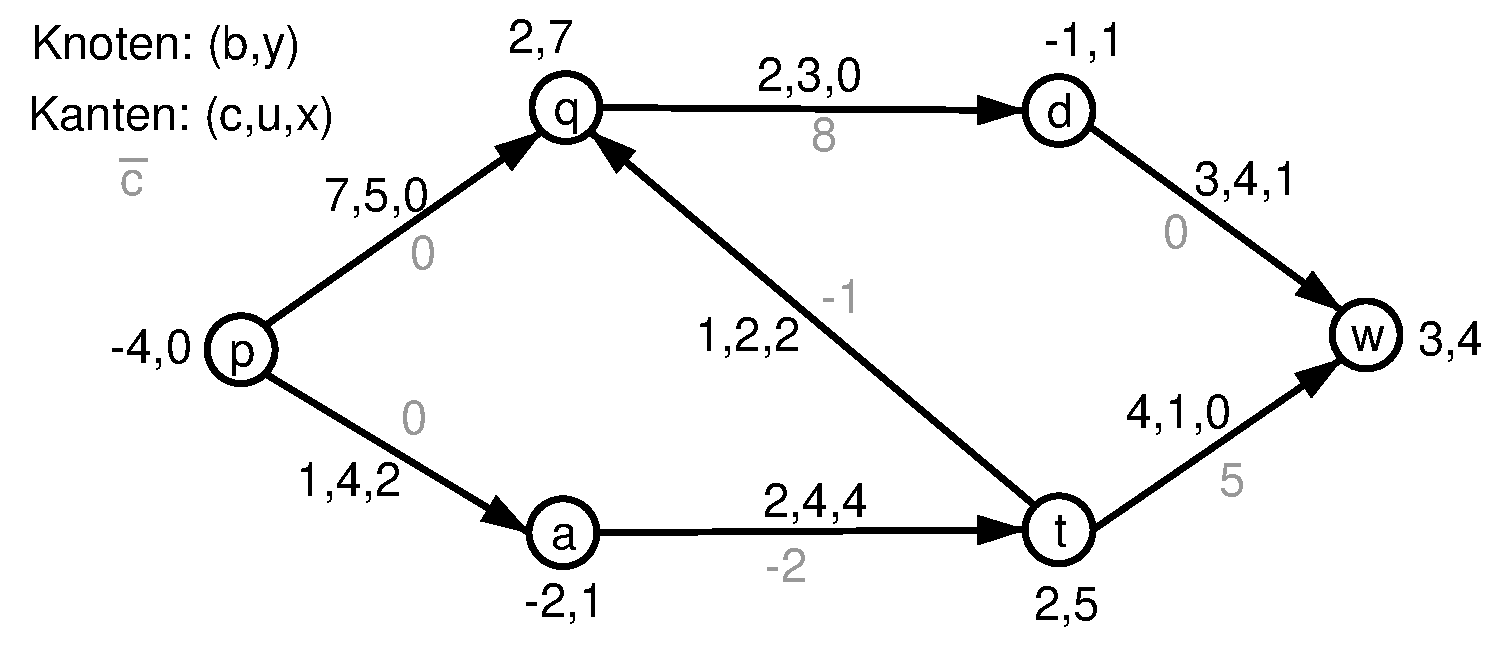
\includegraphics[height=4cm]{bilder/4-3PDMinKostFL}

$p$ ist einzige $x$-Quelle und $w$ ist einzige $x$-Senke.\\
Es sind alle Bedingungen erfüllt $\rightarrow$ Zulässiges Paar $x,\,y$

Suche $x$-erhöhenden Weg von $x$-Quelle zu einer $x$-Senke, Hoffnung: mehr
erfüllte Flussbedingungen.

Begrenzung der Erhöhung $\epsilon$:
\[\begin{array}{rcl}
\epsilon &\leqq& b_{s} - f_{x}(s)\\
\epsilon &\leqq& f_{x}(r)-b_{r}\\
\epsilon &\leqq& \mbox{ Kapazität von P}
\end{array}\]

1. Versuch: $P=p,q,d,w$\\
Erhöhung von $x$ scheitert an $\bc_{q d} = 8 > 0$\\
Analog bei $\bc_{i j} < 0$ kann $x_{i j}$ nicht erniedrigt werden.\\
Also: $P$ darf nur "`Gleichheitskanten"' $e$ haben, d.h. $\bc_{e} = 0$

Annahme $\nexists$ solches $P$\\
$\Rightarrow (\exists R \subseteq V) \; R$ enthält alle $x$-Quellen und
keine $x$-Senken ($R$ enthält alle von einer $x$-Quelle erreichbaren
Knoten auf $x$-erhöhenden Wegen aus Gleichheitskanten) und:
\[\begin{array}{lcl}
e \in \delta(R) &\Rightarrow& \bc_{e} \neq 0 \mbox{ oder } x_{e} = u_{e}\\
e \in \delta(\bar{R}) &\Rightarrow& \bc_{e} \neq 0 \mbox{ oder } x_{e} =
0
\end{array}\]

Im Beispiel $R=\{p,q,a\}$

Definiere Partition:
\[\delta(R) \cup \delta(\bar{R}) = T_{1} \cup T_{2} \cup T_{3} \cup T_{4}\]
mit $\begin{array}[t]{lcl}
T_{1} = \{ e \in \delta(R) | \bc_{e} \leqq 0, \; x_{e} = u_{e}\}\\
T_{2} = \{ e \in \delta(R) | \bc_{e} > 0, \; x_{e} =0\}\\
T_{3} = \{e \in \delta(\bar{R}) | \bc_{e} \geqq 0, \; x_{e} =0\}\\
T_{4} = \{e \in \delta(\bar{R}) | \bc_{e} <0, x_{e} = u_{e}\} 
\end{array}$

Im Beispiel:
\[\begin{array}{rcl}
T_{1}=\{a t\}\\
T_{2}=\{q d\}\\
T_{3}=\varnothing\\
T_{4}=\{t q\}
\end{array}\]

Duale Änderung: Erhöhe $y_{v} \; (v\in \bar{R})$ um $\sigma > 0$\\
$e\in \gamma(R) \cup \gamma (\bar{R})$: $\bc_{e}$ unverändert, mit
$\gamma(R) = $ "`innerhalb R"'\\
$e \in \delta(R): \; \bc_{e} \rightarrow \bc_{e} - \sigma$\\
$e \in \delta(\bar{R}): \; \bc_{e} \rightarrow \bc_{e} + \sigma$\\
$\Rightarrow$ Bedingungen sind noch erfüllt, falls $\begin{array}{l}
\sigma \leqq \bc_{e} \; \; \forall \; e \in T_{2}\\
\sigma \leqq -\bc_{e} \; \; \forall \; e \in T_{4}
\end{array}$

$\sigma$ maximal: Für eine Kante $e\in T_{2} \cup T_{4}$ ist
$\bc_{e}^{\mbox{\footnotesize (neu)}}  = 0$. D.h. $R$ blockt nicht mehr die Suche nach
$x$-erhöhendem Weg mit Gleichheitskanten.

Im Beispiel: $\begin{array}[t]{rcl}\sigma &:=& \min \{\bc_{q d}, \; -\bc_{t q}
\}\\ &=& \min \{8,\, 1\}\\ &=& 1\end{array}$\\
$\Rightarrow t q$ wird Gleichheitskante. 

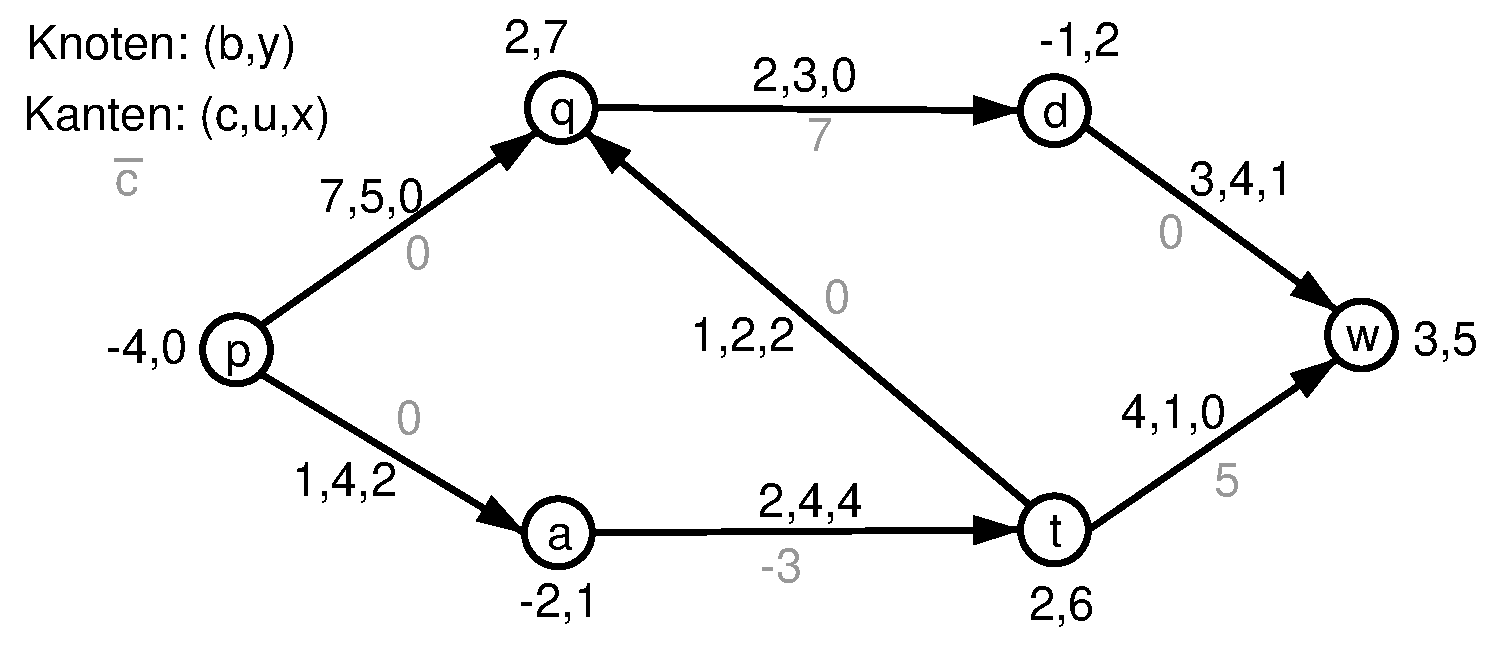
\includegraphics[height=4cm]{bilder/4-3PDMinKostFL2}

zweite Duale Änderung:

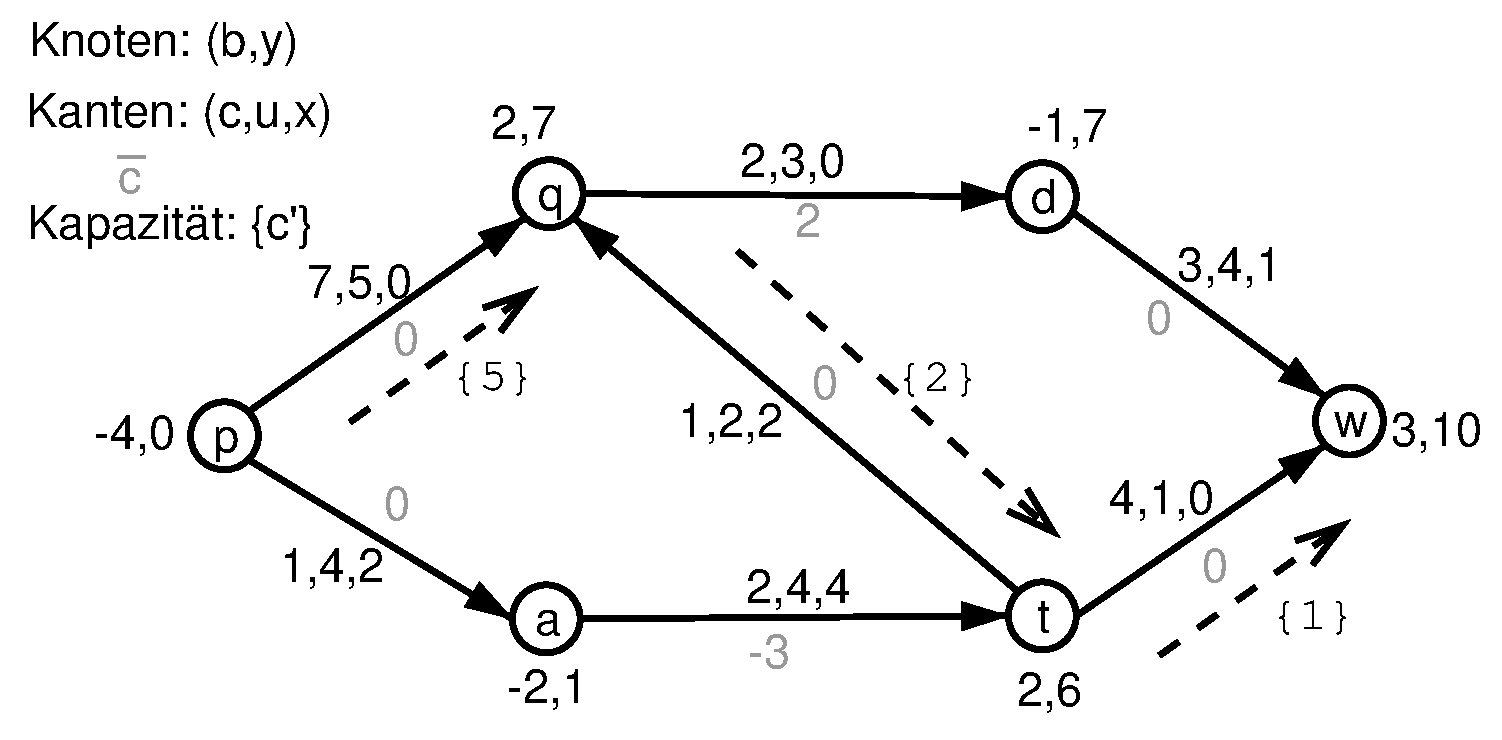
\includegraphics[height=4.4cm]{bilder/4-3PDMinKostFL3}

Also erfolgt eine Flusserhöhung um 1 auf dem Gestrichelten Weg.

Was aber tun, wenn $T_{2}=T_{4} = \varnothing$

Annahme:  $T_{2}=T_{4} = \varnothing$\\
$\bar{R}$ enthält wenigstens eine $x$-Senke und keine $x$-Quelle.\\
\[\begin{array}{rcl}
\Rightarrow b(\bar{R}) &>& \displaystyle \sum_{v \in \bar{R}} f_{x}(v)\\
&=& \underbrace{x(\delta(R))}_{T_{1}} -
\underbrace{x(\delta(\bar{R}))}_{T_{3}}\\
&=& u(\delta(R)) - 0\\
&=& u(\delta(R)) \; \; \mbox{ Widerspruch}
\end{array}\]
Denn Bedarf $\bar{R} >$ Kapazität $R$.\\
Also ist $T_{2} = T_{4} = \varnothing$ unmöglich. Eine duale Änderung
erzeugt immer wenigstens eine neue Gleichheitskante.

\paragraph{Primal Dualer Algorithmus für das Minimum Kosten Flussproblem}
von Ford-Fulkerson, (1956):
\begin{algorithmic}
\STATE Finde $\begin{array}[t]{ll}x,y$ mit $x_{e} = u_{e} & \forall \; e 
\in E \mbox{ mit } \bc_{e} < 0\\
x_{e} = 0 & \forall \; e \in E \mbox{ mit } \bc_{e} > 0\\
0 \leqq x_{e} \leqq u_{e} & \forall \; e \in E\end{array}$\\
\WHILE{($x$ ist nicht zulässig)}
\IF{($\exists$ erhöhender Weg $P$ mit Gleichheitskanten)}
\STATE Finde solches $P$ und erhöhe $x$ auf $P$;
\ELSE
\STATE Finde $\bar{R} \subseteq V$ das alle solche Wege blockt und ändere $y$ für
$\bar{R}$;
\ENDIF
\ENDWHILE
\end{algorithmic}

\begin{itemize}
\item Augmentierungen nach höchstens $n-1$ sukzessiven Änderungen von $y$
\item \# Augmentierungen $\leqq \displaystyle \sum_{\begin{array}{c}v\in V,\\ 
v \mbox{ \footnotesize ist $x$-Senke}\end{array}}  b_{v} - f_{x}(v)$ falls  $u,b$ ganzzahlig.
\end{itemize}

Falls Anfangsfluss $x'$ nicht ganzzahlig dann nur:

\begin{satz}
Falls der P-D-MKFP Algorithmus $x$-erhöhende Wege mit minimaler Kantenzahl
benutzt, so terminiert er nach endlich vielen Schritten.
\end{satz}

Beweis: Übung q.e.d. (Hach, ich liebe diese kurzen Beweise :)

\paragraph{Billigste Augmentierende Wege} \mbox{}\\

Wenn $x$ und $y$ die Bedingungen des P-D--Algorithmus erfüllen, $r,s \in V$
und $P$ ein $x$-erhöhender $(r,s)$-Weg, so hat:

\begin{tabular}{cc} $\begin{array}{rcl }c(P) &= &\displaystyle
\sum_{\begin{array}{c}v w\\\mbox{\footnotesize vorwärts in
$P$}\end{array}} c_{v w}- \sum_{\begin{array}{c}v w\\\mbox{\footnotesize
rückwärts in $P$}\end{array}} c_{v w}\\ &\geqq& \displaystyle
\sum_{\begin{array}{c}v w\\\mbox{\footnotesize vorwärts in
$P$}\end{array}} y_{w} - y_{v} - \sum_{\begin{array}{c}v
w\\\mbox{\footnotesize  rückwärts in $P$}\end{array}}
y_{w}-y_{v}\\ &=& y_{s} - y_{r} \end{array}$& $\begin{array}{rcl}
\multicolumn{3}{l}{\mbox{Vorwärtskanten}}\\ x_{v w} < u_{vw}
&\Rightarrow& \bc_{v w} \geqq 0\\ &\Leftrightarrow&c_{v w} \geqq y_{w}
- y_{v}\\ \multicolumn{3}{l}{\mbox{Rückwärtskanten}}\\ x_{v w} > 0
&\Rightarrow&\bc_{v w} \leqq 0\\ &\Leftrightarrow&c_{w v} \leqq y_{w} -
y_{v} \end{array}$ 
\end{tabular} 
nur Gleichheitskanten in $P$:\\
$c(P) = y_{s}-y_{r}$\\
d.h. $P$ ist billigster augmentierender Weg.

Idee: Finde Augmentierung durch Lösen kürzester Wege Probleme. Kürzeste
Wege Berechnung in G(x), d.h. i.A. negative Kosten: Bellmann-Ford $O(m
n)$.\\
Aber Trick aus Kapitel 2:

Statt $c_{v w}$ Kosten $\bc_{v w} + y_{v} - y_{w}$\\
$\forall \; (r,s)$-Wege $\bc(P)= c(P) + y_{r} -y_{s}$\\
P-D-Bedingungen erfüllt $\Rightarrow$ $G(x)$ hat nicht-negative Kosten,
d.h. wir können Dijkstra anwenden.

Wir müssen die $y$ berechnen.\\
$\sigma_{v} := $ Kosten eines billigsten (bzgl. $\bc$) $x$-erhöhenden Wegs
von einer $x$-Quelle nach $v$ ($=\infty$ falls keiner existiert).\\
Berechnung:

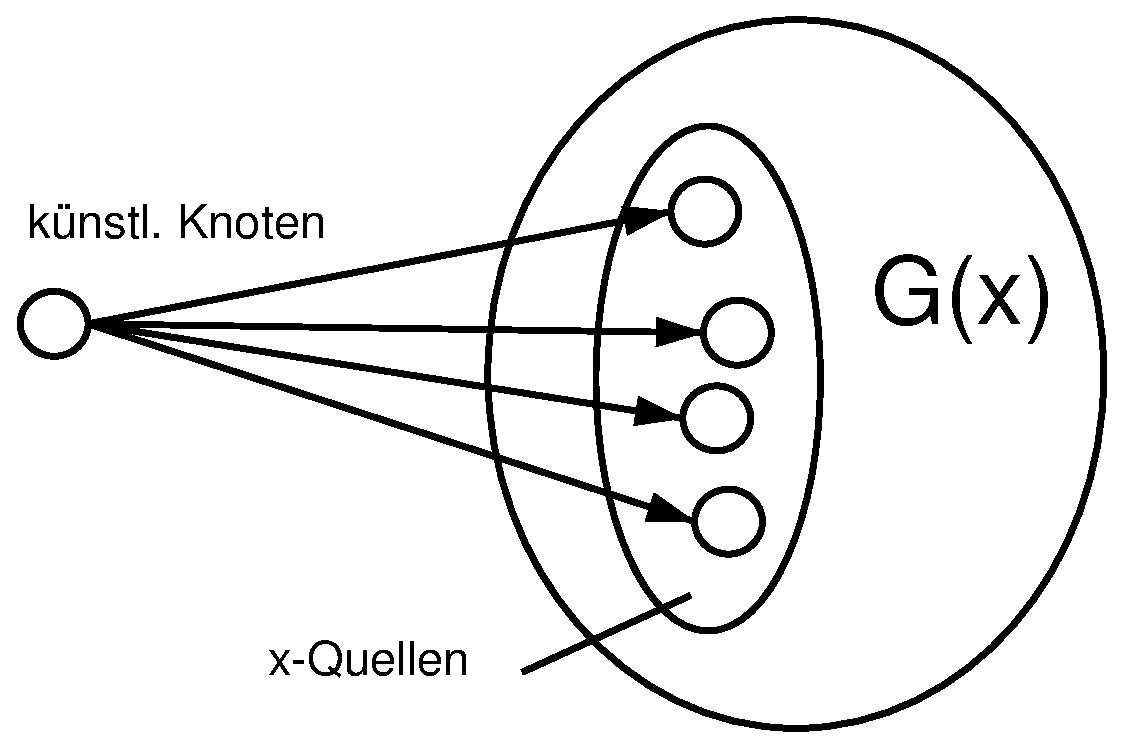
\includegraphics[height=3cm]{bilder/4-3BerechnY}

Augmentierung auf $(r,s)$-Weg $P$ (mit Kosten $\bc$ berechnet).\\
Es gilt für alle Vorwärtskanten $v w$ in $P$:
\[\begin{array}{ll}
&\sigma_{v} + \bc_{v w} = \sigma_{w}\\
\Rightarrow&c_{v w} + y_{v} - y_{w} + \sigma_{v} - \sigma_{w} = 0\\
\Rightarrow& (c_{v w} + y_{v} + \sigma_{v}) - (y_{w} + \sigma_{w}) = 0
\end{array}\]
Gleiches gilt für die Rückwärtskanten analog.\\
Also für $y'_v := y_{v} + \sigma_{v}$ ist $P$ ein Weg mit
Gleichheitskanten.\\
$\Rightarrow x'$ neues $x$  und $y'$ erfüllen die P-D-Bedingungen für alle
$e \in P$.\\
(andere Kanten ?) 

\subsection{Primal-Dualer Algorithmus mit billigsten augmentierenden Wegen}
\begin{algorithmic}
\STATE Finde $x,y$ die P-D-Bedingungen erfüllen;
\WHILE{($x$ ist nicht zulässig)}
\STATE Finde für alle $v\in V$ einen bezüglich $\bc$ billigsten
$x$-erhöhenden Weg $P_{v}$ von einer $x$-Quelle zu $v$;
\STATE $\sigma_{v} := $ Kosten von $P_{v}$ ($\infty$, falls $\nexists
\; P_{v}$);
\STATE Wähle $x$-Senke mit minimalem $\sigma_{s}$;
\STATE Augmentiere $x$ auf $P_{s}$;
\STATE Für alle $v\in V$ $y_{v} \leftarrow y_{v} + \min\{\sigma_{v},
\sigma_{s}\}$;
\ENDWHILE
\end{algorithmic}

\begin{lemma}
$x$ und $y$ im P-D-Algorithmus mit billigsten augmentierenden Wegen erfüllt
die P-D-Bedingungen.
\end{lemma}

Beweis:\\
$(x,y) \rightarrow (x',y')$, $(x,y)$ erfüllt die P-D-Bedingungen.

Zu Zeigen: $(x',y')$ erfüllt P-D-Bedingungen.\\
$0\leqq x_{e} \leqq u_{e}$ bleiben bei jeder Augmentation erhalten.\\
Komplementäre Schlupfbedingungen gelten für alle $e\in P_{s}$

Sei $v w \not\in P \Rightarrow x'_{v w} = x_{v w}$\\
Z.Z.:
\begin{itemize}
\item[] (a) $x_{v w} \leqq u_{v w} \Rightarrow c_{v w} + y'_{v} - y'_{w}
\geqq 0$
\item[] (b) $x_{v w} > 0 \Rightarrow c_{v w} + y'_{v} - y'_{w} \leqq 0$ 
\end{itemize}

\begin{itemize}
\item[(a)]
\begin{enumerate}
\item Fall: $\sigma_{v} \leqq \sigma_{s}$\\
\[\begin{array}{rcl}
c_{v w} + y'_{v} - y'_{w} &=& \bc_{v w} - y_{v} + y_{w } + y'_{v} - y'_{w}\\
&=& \bc_{v w} - y_{v} + y_{w} + y_{v} + \min\{\sigma_{v}, \sigma_{s}\} -
y_{w} - \min\{\sigma_{w},\sigma_{s}\}\\
&=& \bc_{v w} + \min\{\sigma_{v},\sigma_{s}\} -
\min\{\sigma_{w},\sigma_{s}\}\\
&\stackrel{\sigma_{v} < \sigma_{s}}{=}& \bc_{v w} + \sigma_{v} -
\min\{\sigma_{w},\sigma_{s}\}\\
&\geqq& \bc_{v w} + \sigma_{v} - \sigma_{w}\\
&\geqq& 0
\end{array}
\]
\item Fall: $\sigma_{v} \geqq \sigma_{s}$
\[\begin{array}{rcl}
c_{v w} + y'_{v} - y'_{w} &=& \bc_{v w} + \min\{\sigma_{v},\sigma_{s}\} -
\min\{\sigma_{w},\sigma_{s}\}\\
&\stackrel{\sigma_{v} \geqq \sigma_{s}}{=}& \bc_{w} + \underbrace{
\sigma_{s} - \min\{\sigma_{w},\sigma_{s}\}}_{\geqq 0}\\
&\geqq& \bc_{v w}\\
&\geqq& 0
\end{array}\]
\end{enumerate}
$x,y$ erhalten P-D-Bedingungen
\item[(b)] analog q.e.d.
\end{itemize}

\begin{satz}
Sind $b$ und $u$ ganzzahlig, $x$ der ganzzahlige Ausgangsfluss, und
\[B_{x} = \sum_{\begin{array}{c}v \in V\\\mbox{\footnotesize $v$ $x$-Senke}\end{array}
} (b_{v} - f_{x}(v))\]
so löst der primal-duale Algorithmus mit billigsten augmentierenden Wegen
das Minimum-Kosten-Flussproblem  in Zeit $O(S(n,m)B_{x})$.

Spezialfall Transshipment: Der Anfangsfluss kann als 0-Fluss gewählt
werden, d.h:
\[B_{x} = B = \sum_{\begin{array}{c}v \in V\\b_{v} > 0\end{array}} b_{v}\]
\end{satz}

\begin{lemma}
Ist $b$ ganzzahlig, so löst der primal-duale Algorithmus mit billigsten
augmentierenden Wegen das Transshipment-Problem in Zeit $O(S(n,m)B)$.
q.e.d.
\end{lemma}
Anm.: also kein polynomieller Algorithmus

\section{Skalierungsalgorithmen für das MKFP}
Annahmen:
\begin{itemize}
\item Transshipment ($u_{e} = \infty \; \forall \; e \in E$) (O.B.d.A.)
\item $b_{v} \in \ZZ \; \forall v \in V$
\item Existenz einer Optimallösung gesichert (O.B.d.A.)
\item $(\exists r \in V) \; b_{r} = 0$
\[(\forall \; v \in V \wout \{r\}) \; r v \in E, \; v r \in E, c_{v r} = 0\]

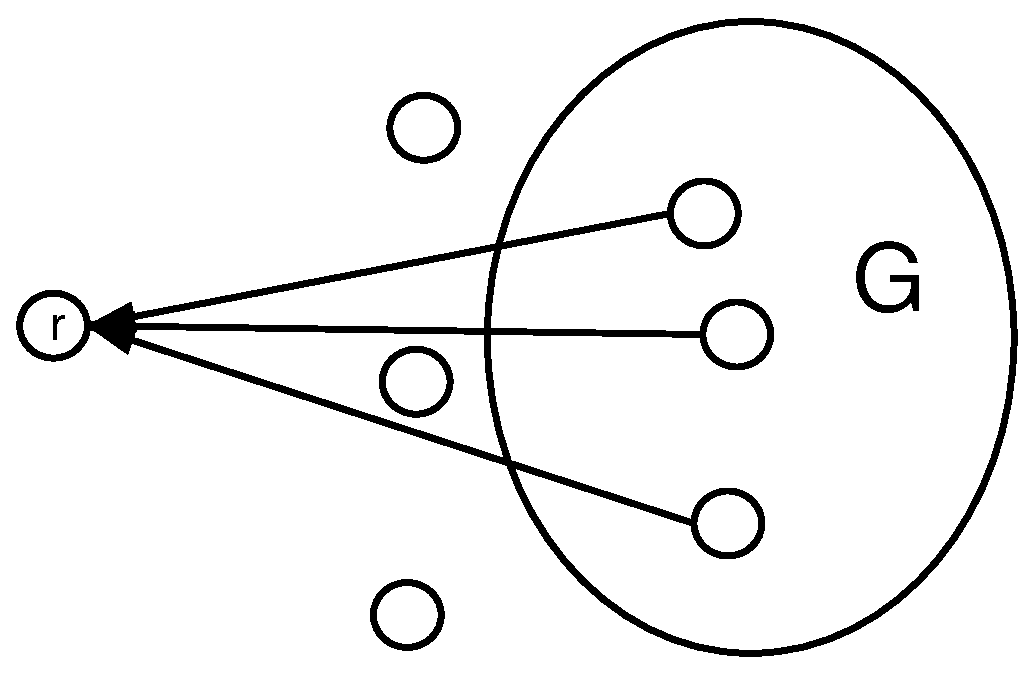
\includegraphics[height=3cm]{bilder/4-4Skalierung1}
\end{itemize}
In jeder zulässigen Lösung $x_{v r} = 0$ d.h. O.B.d.A.

\paragraph{Skalierung von $(G,c,b)$ mit $\Delta >0$}:\\
$b_{v} \rightarrow b'_{v} = \left\lfloor \frac{b_{v}}{\Delta}\right\rfloor
\; \; \forall \; v \in V \wout \{r\}$\\
$b_{r} \rightarrow b'_{r} = - b'(V \wout \{r\})$\\
$\Rightarrow b'(v) = 0$\\
Beispiel:

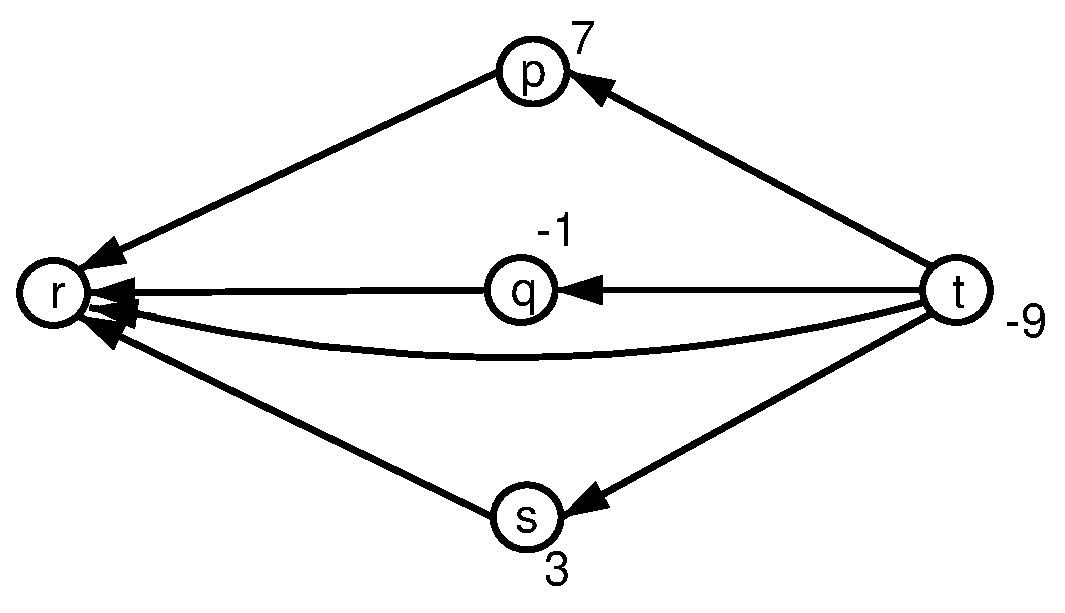
\includegraphics[width=4cm]{bilder/4-4Skalierung2} 
$\stackrel{\Delta=4}{\rightarrow}$ 
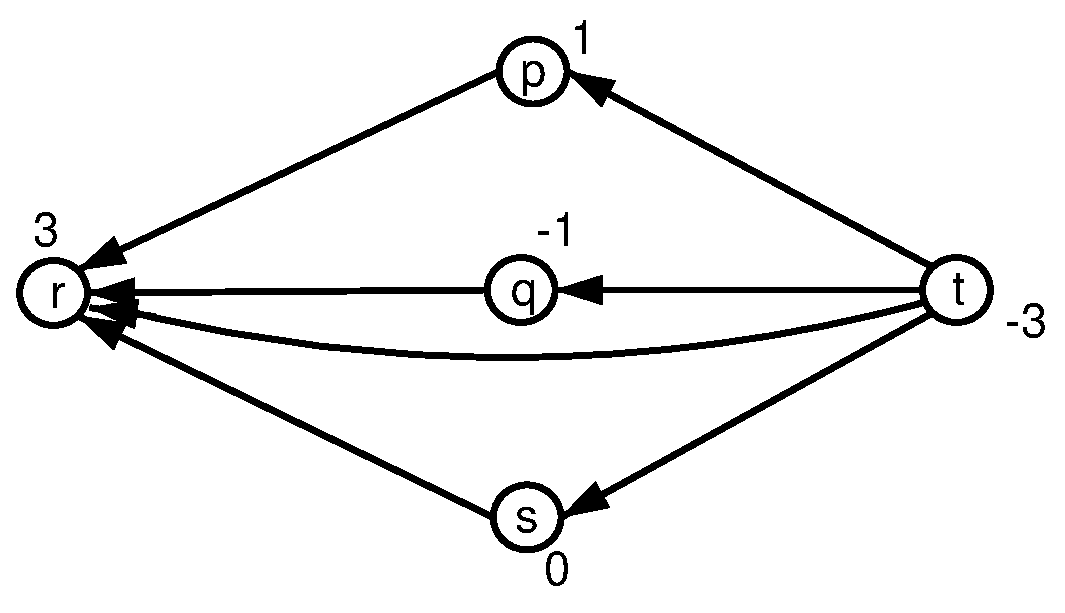
\includegraphics[width=4cm]{bilder/4-4Skalierung3}

\begin{lemma}
Hat $(G,c,b)$ eine Optimallösung, so auch jede Skalierung von $(G,c,b)$
\end{lemma}
Beweis:\\
$\begin{array}{ccc}
(G,c,b)&\stackrel{\mbox{\footnotesize Skaliert mit
$\Delta$}}{\longrightarrow}&(G,c,b')\\
\mbox{\footnotesize kein negativer}&&\mbox{\footnotesize kein negativer}\\
\mbox{\footnotesize gerichteter Kreis}&&\mbox{\footnotesize gerichteter
Kreis}
\end{array}$

$\Rightarrow (G,c,b')$ ist nicht unbeschränkt, d.h. zu zeigen $(G,c,b')$ hat
eine zulässige Lösung.

Der Übergang zur nächsten Aussage wurde mit einem langen Handout von Herrn
Professor Jünger gezeigt, dieses sei an dieser Stelle nun zitiert:

\begin{quote}
In Übungsaufgabe 36 wurde gezeigt, dass die Zulässigkeit von
\[\begin{array}{rcl@{\hspace{6mm}}l}
f_x(v) &=& b_v& \forall \; v \in V\\
0 \leq x_e &\leq& u_e& \forall \; e \in E
\end{array}\]
für $G=(V,E)$ und $b(V)=0$ mit Hilfe einer Maximum-Fluss-Berechnung
entschieden werden kann. Eine Lösung besteht in der Definition eines
Hilfsdigraphen $G'$:

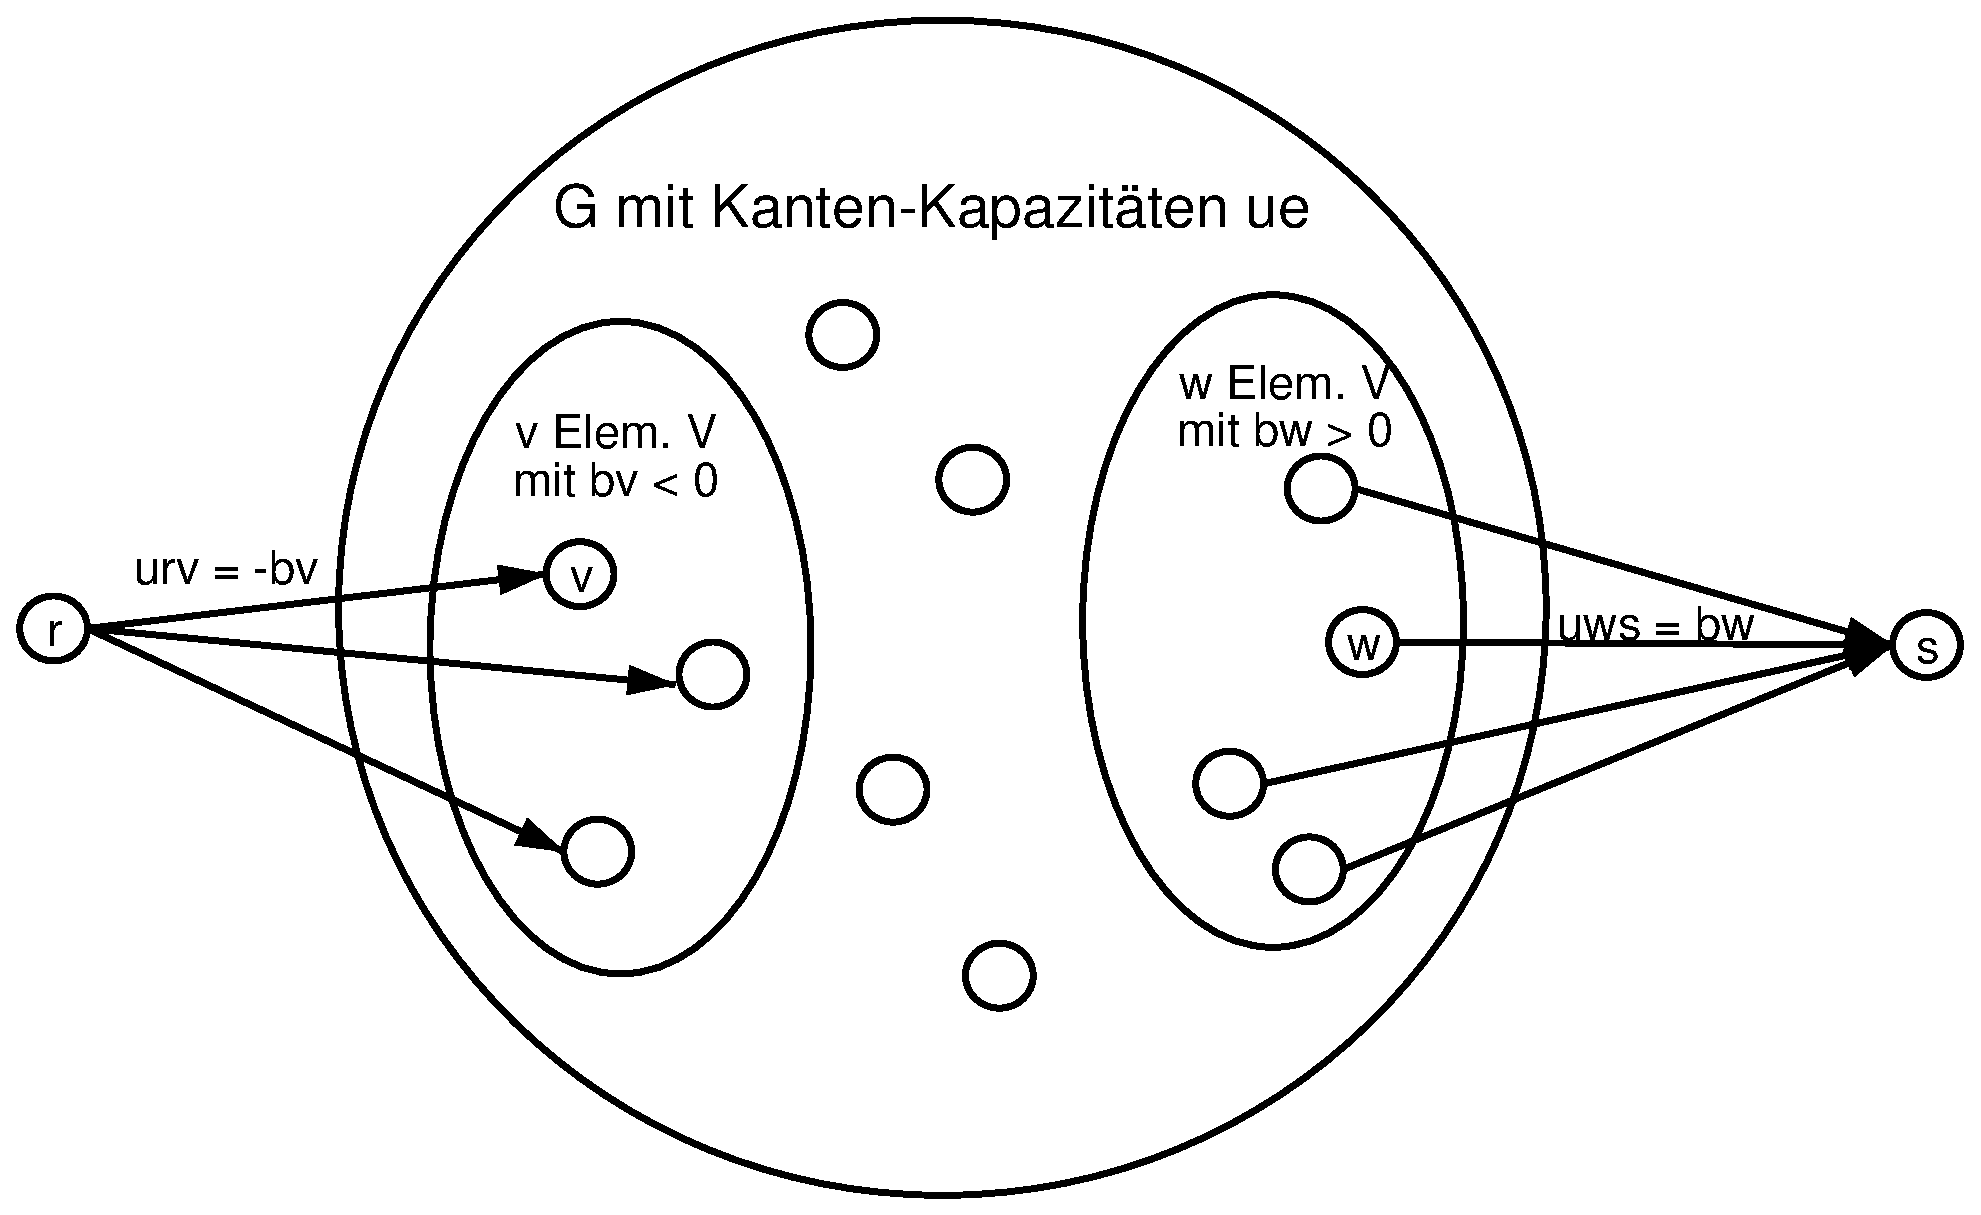
\includegraphics[height=6cm]{bilder/4-4Handout}

Dann gilt offensichtlich:
\[\begin{array}{rcl@{\hspace{6mm}}l}
(\exists x) \; \; f_x(v) &=& b_v &\forall \; v \in V\\
0 \leq x_e &\leq& u_e & \forall \; e \in E
\end{array}
\]
genau dann, wenn $b(v) = 0$ und $\exists$ $(r,s)$-Fluss in $G'$ mit
Flusswert $\displaystyle \sum_{v\in V,\; b_{v}>0} b_{v}$.

Wir können daraus eine andere notwendige und hinreichende Bedingung
herleiten:

$\exists$ $(r,s)$-Fluss in $G'$ mit Flusswert $\displaystyle \sum_{v \in
V,\; 
b_{v} > 0} b_v$ genau dann, wenn $b(v) = 0$ und 
\[(\nexists A \subseteq V) \; \; u(\delta'(A \cup \{r\})) < \sum_{v \in V, \;
b_v > 0} b_v (\mbox{Max-Flow-Min-Cut})\]
genau dann, wenn $b(v) = 0$ und:
\[ (\nexists A \subseteq V) \; \; u(\delta(A)) + \sum_{v \not\in A, \; b_v
< 0}(-b_v) + \sum_{v \in A, \; b_v >0} b_v <  \sum_{v \in V, \; b_v > 0}
b_v\]
genau dann, wennn $b(v)=0$ und
\[\begin{array}{rcl}
 (\nexists A \subseteq V) \; \; u(\delta(A)) &< &\displaystyle \sum_{v \in V, \; b_v > 0}
b_v - \sum_{v \in A, \; b_v >0} b_v +  \sum_{v \not\in A, \; b_v
< 0} b_v\\
&=& \displaystyle  \sum_{v \not\in A, \; b_v > 0} b_v +  \sum_{v \not\in A,
\; b_v < 0} b_v\\
&=& \displaystyle \sum_{v \not\in A} b_v
\end{array}\]
genau dann, wenn $b(v)=0$ und 
\[(\forall \; A \subseteq V) \; \; b(A) \leq u(\delta(\bar{A}))\]
Es gilt also der\\
{\bf Satz}
\[\begin{array}{rcl@{\hspace{6mm}}l}
(\exists x) \; \; f_x(v) &=& b_v&\forall \; v \in V\\
0\leq x_e &\leq&u_e&\forall \; e \in E
\end{array}\]
genau dann, wenn $b(v) = 0$ und $(\forall \; A \subseteq V) \; \; b(A) \leq
u(\delta(\bar{A}))$.

Für den Spezialfall des Transshipment-Zulässigkeitsproblems ($u_e=\infty$
$\forall \; e \in E$) folgt sofort das\\
{\bf Korollar}
\[\begin{array}{rcl@{\hspace{6mm}}l}
(\exists x) \; \; f_x(v) &=& b_v&\forall \; v \in V\\
x_e &\geq&0&\forall V \in E
\end{array}\]
genau dann, wenn $b(v) = 0$ und
\[(\forall \; A \subseteq V) \; \; \delta(\bar{A}) = \varnothing
\Rightarrow b(A) \leq 0\]
(Falls $b$ (und $u$) ganzzahlig sind, gelten Satz und korollar auch mit
ganzzahligem $x$)
\end{quote}

Soviel zum Zitat, weiter in der Vorlesung

$(\forall\; A \subseteq V)\;  \delta(\bar{A}) = \varnothing \Rightarrow
b'(A) \leqq 0$\\
\[\begin{array}{rclcl}
\delta(\bar{A}) = \varnothing &\Rightarrow& r \in \bar{A}\\
&\Rightarrow& b'(A) &=& \displaystyle \sum_{v \in A} \left\lfloor
\frac{b_{v}}{\Delta}\right\rfloor\vspace{2mm}\\
&&&\leqq& \displaystyle \sum_{v \in A} \frac{b_{v}}{\Delta}\vspace{2mm}\\
&&&=&\frac{b(A)}{\Delta}
\end{array}
\]
Daraus und $(G,c,b)$ hat eine zulässige Lösung $\Rightarrow b(A) \leqq 0$
folgt: Auch $b'(A) \leqq 0$. q.e.d.

\subsubsection{Schrittweise Skalieren nach Edmonds und Karp [1972]}

Genannt: "`successive scaling"'

Für $k > 0$ sei $(G,c,b^k)$ die Skalierung von $(G,c,b)$ mit $\Delta =
2^k$. (Entfernen der $k$ letzten Bits in der Dualdarstellung.)\\
$b^0 = b$\\
$(x',y')$ sei ein Paar von optimalen primalen/dualen Lösungen für
$(G,c,b^{k+1})$.\\
$\Rightarrow x = 2x'$, $y=y'$ erfüllen die P-D-Bedingungen für $(G,c,b^k)$.\\
$x_e \geqq 0$ und $\underbrace{x_e=0}_{\mbox{\footnotesize für $(G,c,b^k)$}}
 \; \; \forall \; e \in E$ mit $\bc_e > 0$

Für $v\neq r$ mit $V=V_{1} \cup V_{2} \cup \{r\}$ gilt:
\[\begin{array}{rcll}
b_{v}^k &=&b^{k+1}_v& v \in V_{1}\\
\mbox{oder: }b_{v}^k &=&b_{v}^{k+1} + 1& v\in V_2\\
\end{array}
\]
\[\begin{array}{rcl}
\Rightarrow b_{r}^k &=& - \displaystyle \sum_{v\in V_1} 2b_{v}^{k+1}
-\sum_{v\in V_{2}} (2b^{k+1}_v +1)\\
&=& - \displaystyle \sum_{v\in V} 2b^{k+1}_v - | V_2|\\
&=& 2b^{k+1}_r - |V_2| \leqq 2b^{k+1}_r
\end{array}
\]
\[\rightarrow\sum_{\mbox{\scriptsize\begin{tabular}{cc}$b_{v}^k > f_x(v)$\\$v$ ist
$x$-Senke\end{tabular}}}
b_{v}^k -f_x(v) \leqq n-1\]
D.h. der P-D-Algorithmus mit Startlösung $(x,y)$ löst $(G,c,b)$ durch
höchstens $n-1$ nicht-negative-Kosten-kürzeste-Wege-Berechnungen.

\subsubsection{Schrittweiser Skalierungsalgorithmus für das Transshipment
Problem}
\begin{algorithmic}
\STATE $K := \min \{k | |b_v| \leqq 2^k \; \; \forall \; v \in V\}$; Anzahl
der Bits im längsten $b_v$
\STATE $x:= 0$;
\FOR{($k:= K, K-1, K-2,\ldots,1$)} 
\STATE löse $(G,c,b^k)$ mittels P-D-Algorithmus mit Startlösung $(2x,y)$;
\STATE Sei $(x,y)$ primal/duale Optimallösung;
\ENDFOR
\end{algorithmic}

\begin{satz}
Sei $(G,c,b)$ eine Instanz des Transshipment-Problems und $b\in \ZZ^V$mit
Optimallösung. Dann löst der schrittweise Skalierungsalgorithmus $(G,c,b)$
in Zeit $O(n\, S(n,m)(1+\log B))$ mit:
\[B=\sum_{\mbox{\scriptsize\begin{tabular}{c}$v\in
V$\\$b_v>0$\end{tabular}}} b_v\]
\end{satz}
Beweis:\\
$k<K$: P-D-Algorithmus mit $O(n)$ kürzeste-Wege-Berechnungen (vorhin).\\
\[\begin{array}{rcl}(G,c,b^k):\; \; \displaystyle \sum_{b_{v}^k>0} b_{v}^k 
&=& - \displaystyle \sum_{b_{v}^k<0} b_{v}^k\\
&=& |\{v| b_v < 0\}| = O(n) \end{array}\]
D.h. zusammen $\leqq (K+1)n$ kürzeste-Wege-Berechnungen. $K+1 \leqq 1 +
\lceil \log (\max|b_v|)\rceil \leqq 2 + \log B$ q.e.d.

Polynomieller Algorithmus für Transshipment-Problem führt zu polynomiellen
Algorithmus für MKFP. Leider gehen die Zahlen $b_v \; (v\in V)$ in die
Laufzeitschranke ein. Edmonds und Karp [1972] fragten, ob es einen {\em
stark polynomiellen Algorithmus} für
das MKFP gibt (polynomielle Laufzeitfunktion in $n=|V|$ und $m=|E|$).

Diese Frage wurde 1985 von Eva Tardos mit "`ja"' beantwortet. Die Details
der resultierenden "`Skalier- und Kontraktionsalgorithmen"' sind
kompliziert, hier aus Zeitgründen, nur das beste Resultat.

\begin{satz}
Aufgestellt von Orlin [1988]: Ein gewisser "`Skalier und
Kontraktionsalgorithmus"' löst das Minimum-Kosten-Flussproblem in Zeit $O(m
\log n \, S(n,m))$.

\end{satz}





